\documentclass[22pt]{report}
\usepackage{graphicx}
\usepackage{blindtext}
\usepackage{geometry}
\usepackage{caption}
\usepackage{subcaption}
\usepackage{geometry}
\usepackage{amsmath}
\usepackage{amssymb}
\usepackage{tabularx}
\usepackage{lipsum}
\usepackage{xcolor}
\usepackage{chronology}
\usepackage{subfig}
\usepackage{hyperref}
\renewcommand{\arraystretch}{1.5}

\geometry{
	a4paper,
	right=15mm,
	bottom=20mm,
	left=15mm,
	top=20mm,
}
\title{Stereo Vision}

\author{
Dr. Sabzi \\ Advisor \\\\
% Prof. Dr. Markus Klute \\ Supporting Professor 
% \and 
% Prof. Dr. Frank Simon \\ Supporting Professor 
% \and
% Sören Finna \\ BSc Student
% \and 
Ahmadreza Khanari \\ BSc Student \\ \\
Leili Motahari \\ BSc Student}

\date{2024}

\begin{document}
\begin{figure}
	
\includegraphics[width=0.4\linewidth]{Images/Sharif-eng-logo}
	\label{Shariflogo}
	\centering
        % \caption*{Sharif University of Technology}
\end{figure}

\maketitle
\tableofcontents
\setcounter{chapter}{0}

\chapter{Preamble}
    \section{What is Stereo Vision} 
        Stereo vision, also known as stereoscopic vision, refers to the ability to perceive depth and three-dimensional structure of an environment based on visual information derived from two slightly different viewpoints. This concept is primarily based on the biological phenomenon of binocular vision found in humans and many animals, where each eye captures its own view and the brain combines these two images into a single, three-dimensional perception.
        \newline
    
        \begin{figure}[h]
            \centering
            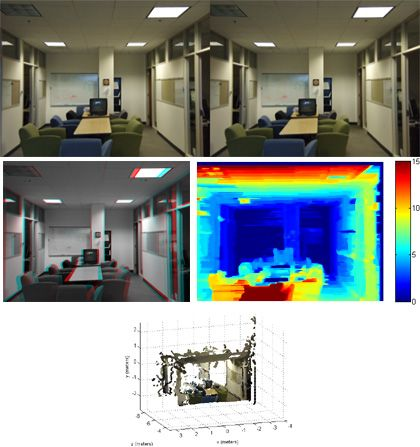
\includegraphics[width=0.5\linewidth]{Images/WhatIsIt.jpg}
            \caption{Stereo Vision}
            \label{fig:enter-label}
        \end{figure}

        
    % \section{Tentative timeline}
    % \begin{tabularx}{\textwidth} { 
    % 		| >{\centering\arraybackslash\bf}X 
    % 		| >{\raggedright\arraybackslash}X 
    % 		| >{\raggedright\arraybackslash}X | }
    % 	\hline
    % 	Period / Date & \bf{Phase} & \bf{Comments} \\
    % 	\hline
    % 	  16 June - 1 July  & Publicity \& Application & -  \\
    % 	\hline
    % 	  1 July  & Proposal & Feedback about proposal  \\
    % 	\hline
    % 	1 June - 30 July  & Detailed proposal  & Details about resources  \\
    % 	\hline
    % 	30 July  & Project confirmation  & Approval by Professors  \\
    % 	\hline
    % 	1 August - 8 November  & Official IRIS Period  & Deliverables due by 8 November\\
    % 	\hline
        
    % \end{tabularx}

    \section{Applications of Stereo Vision}
        Stereo vision is not just a natural biological phenomenon but also a concept applied in various technological fields:
        \begin{enumerate}
            \item \textbf{Robotics}\\
                Robots use stereo vision for navigation, object recognition, and complex tasks like manipulation. It helps them determine the positions and sizes of objects in their environment.
                \begin{itemize}
                    \item\textbf{Navigation and Obstacle Avoidance}\\
                        Robots equipped with stereo vision can navigate complex environments by detecting and avoiding obstacles. This is crucial in environments like warehouses, outdoor landscapes, and even on other planets (as seen in Mars rovers).\\
                    \item \textbf{Object Manipulation}\\
                        In industrial settings, robots use stereo vision to pick up and assemble parts accurately. This is essential in automated production lines where precision is critical.
                \end{itemize}
            \item \textbf{Autonomous Vehicles}\\
                Self-driving cars use stereo vision systems to identify obstacles, measure distances, and make navigation decisions.
                \begin{itemize}
                    \item \textbf{Safe Navigation}\\
                        Self-driving cars use stereo vision to detect the distances of vehicles, pedestrians, and other obstacles. This depth information helps in making critical driving decisions, like braking or steering to avoid collisions.
                    \item \textbf{Road Condition Monitoring}\\
                        Stereo vision can help in assessing road conditions by detecting potholes, barriers, and uneven surfaces, contributing to safer driving strategies.
                \end{itemize}
            \item \textbf{3D Movies, Virtual Reality (VR) and Augmented Reality (AR)}\\
                 Stereo vision technology is used to create immersive experiences in movies and VR by presenting slightly different images to each eye, creating a sense of depth.
                 \begin{itemize}
                     \item \textbf{Enhanced Immersion}\\
                         In VR, stereo vision is used to create a deep immersive experience by presenting two slightly different images to each eye, mimicking natural human vision.
                     \item \textbf{Interactive Experiences}\\
                         In AR, stereo vision helps overlay digital content onto the real world in a way that it appears to coexist in three-dimensional space, enhancing user interaction.
                 \end{itemize}   
            \item \textbf{Film and Photography}\\
                 This is used in mapping and surveying, where stereo vision helps in calculating the positions of points in space, based on images taken from different locations.
                 \begin{itemize}
                     \item \textbf{3D Movies} \\
                         Filmmakers use stereo cameras to shoot scenes from two slightly different angles, creating a depth effect that is viewed using 3D glasses.
                    \item \textbf{Photogrammetry}\\
                        Used in archaeology and geology, stereo vision allows for the reconstruction of 3D models from photographs taken from different angles.
                 \end{itemize}
            \item \textbf{Medical Imaging}\\
                 Techniques like stereoscopic endoscopy allow doctors to perceive depth in images, enhancing their ability to perform precision surgeries.
                 \begin{itemize}
                    \item \textbf{Surgical Assistance}\\
                        In minimally invasive surgery, stereo vision provides surgeons with a three-dimensional view of the operating area, improving precision and outcomes.
                    \item \textbf{Diagnostic Tools}\\
                        Stereo vision techniques are used in ophthalmology to assess the 3D structure of the eye and in dentistry for accurate 3D imaging of teeth.
                 \end{itemize}
            \item \textbf{Surveillance and Security}
                \begin{itemize}
                    \item \textbf{Enhanced Monitoring}\\
                        Stereo vision can be used in security systems to estimate the size and speed of people or objects, enhancing motion detection and threat assessment.
                \end{itemize}
            \item \textbf{Sports and Entertainment}
                \begin{itemize}
                    \item \textbf{Athlete Training}\\
                        Stereo vision systems analyze the movements of athletes to enhance performance and reduce injury risks.
                    \item \textbf{Event Broadcasting} \\
                        Stereo vision can be applied to provide viewers with a three-dimensional viewing experience of live events.
                \end{itemize}
            \item \textbf{Consumer Electronics}
                \begin{itemize}
                    \item \textbf{Gaming}\\
                        Some gaming systems use stereo vision to track player movements and gestures, creating more interactive gameplay.
                    \item \textbf{Smartphones} \\
                        Newer models incorporate depth sensors that use stereo vision principles to enhance photo capabilities and AR experiences.
                \end{itemize}
        \end{enumerate}

    \section{The applications of Stereo vision in agriculture}
        Stereo vision technology holds significant potential for agriculture, enhancing various aspects from monitoring to automation. Here are some key applications of stereo vision in the agricultural sector:
        \begin{enumerate}
            \item \textbf{Precision Farming}
                \begin{itemize}
                    \item \textbf{Crop Monitoring} \\
                        Stereo vision systems can be used to capture detailed 3D images of crops across large fields. By analyzing these images, farmers can assess plant health, growth patterns, and detect anomalies like diseases or pests at early stages.
                    \item \textbf{Water Management}\\
                        By assessing the terrain and crop canopy in 3D, stereo vision helps in optimizing irrigation strategies, ensuring water is distributed efficiently and effectively according to the landscape and crop needs.
                \end{itemize}
            \item \textbf{Agricultural Robotics}
                \begin{itemize}
                    \item \textbf{Automated Harvesting}\\
                        Robots equipped with stereo vision can identify ripe fruits and vegetables, assessing their size and ripeness. This allows for precise picking, reducing damage to the produce and plants.
                    \item \textbf{Weeding and Planting}\\
                        Stereo vision helps agricultural robots distinguish between crops and weeds, enabling targeted weeding operations. It also assists in accurate planting, ensuring seeds are placed at optimal depths and spacing.
                \end{itemize}
            \item \textbf{Phenotyping}
                 \begin{itemize}
                     \item \textbf{Plant Trait Analysis}\\
                        Stereo vision is used in high-throughput plant phenotyping where it helps in measuring physical traits of plants such as leaf area, plant height, and biomass. This is crucial for breeding and research purposes, enabling the selection of superior crop varieties.
                 \end{itemize}       
            \item \textbf{Terrain and Field Analysis}
                 \begin{itemize}
                     \item \textbf{Soil and Field Assessment}\\
                        3D mapping of fields using stereo vision helps in understanding soil variations, terrain features, and other critical factors that influence agricultural practices. This data can be used to optimize field layouts, planting patterns, and manage resources more effectively.
                 \end{itemize}
            \item \textbf{Livestock Management}
                 \begin{itemize}
                     \item \textbf{Behavior and Health Monitoring}\\
                        In livestock management, stereo vision can help monitor animal behavior and movements, detecting signs of illness or distress early. This technology can provide 3D spatial data that helps in assessing the condition of livestock and their living environments.
                 \end{itemize}
            \item \textbf{Drone and Aerial Imaging}
                \begin{itemize}
                    \item \textbf{Aerial Surveys}\\
                        Drones equipped with stereo vision cameras can perform detailed 3D surveys of agricultural land. This aerial perspective is invaluable for large-scale monitoring, crop scouting, and managing crop health at a macro level.
                \end{itemize}
            \item \textbf{Storage and Logistics}
                \begin{itemize}
                    \item \textbf{Volume Estimation}\\
                        Stereo vision helps in estimating the volume of stored grains and other agricultural products, facilitating better storage and logistics management. This can be crucial for inventory control and planning.
                \end{itemize}
        \end{enumerate}
        By integrating stereo vision into these areas, agriculture can achieve higher precision, efficiency, and productivity, addressing challenges such as labor shortages, sustainability issues, and the increasing demand for food due to global population growth.


    \section{Technical Implementation}
        In technology, stereo vision often involves using two cameras (mimicking the human eyes) placed at a certain distance apart. Each camera captures a scene from its own viewpoint. Sophisticated algorithms then analyze the differences between these two images to reconstruct a 3D scene. The process involves steps like image rectification, disparity computation, and sometimes machine learning techniques to enhance the depth perception accuracy.
        Overall, stereo vision is a fascinating blend of biology and technology, offering essential insights into how we perceive our three-dimensional world and providing critical capabilities in various modern applications.

    \section{What is the difference between monocular and stereo image?}
        The main difference between monocular and stereo imaging lies in the number of cameras used and the resulting capabilities, particularly in terms of depth perception. Here's a detailed look at both approaches:\\\\
        \textbf{Monocular Vision}\\\\
        \textbf{Definition:} Monocular vision involves the use of a single camera to capture images. Since it mimics the human capability of using one eye, it offers a flat, two-dimensional view of the world.\\
        \textbf{Characteristics:}
        \begin{itemize}
            \item \textbf{2D Perception:} Monocular systems provide two-dimensional images.
            \item \textbf{Simplicity and Cost:} Using a single camera makes monocular systems simpler and often cheaper than stereo systems.
            \item \textbf{Depth Estimation:} Depth information is not directly available and must be inferred using techniques that analyze motion, perspective, and other visual cues.
            \item \textbf{Applications:} Common in photography, video recording, and some forms of robotics and autonomous vehicle guidance where depth is either not critical or can be estimated through other means.\\
        \end{itemize}
        \textbf{Stereo Vision}\\\\
        \textbf{Definition:}
        Stereo vision uses two cameras, typically positioned a small distance apart (similar to human eyes), to capture slightly different images of the same scene.\\
        \textbf{Characteristics:}
        \begin{itemize}
            \item \textbf{3D Perception:} By comparing the differences between the two images (a process known as stereo matching), depth information can be directly calculated, providing a three-dimensional perception of the scene.
            \item \textbf{Complexity and Cost:} Stereo systems are more complex and typically costlier than monocular systems due to the need for two cameras and more sophisticated computational techniques.
            \item \textbf{Direct Depth Measurement:} Stereo vision can measure the depth and distances of objects directly from the disparities between the images captured by the two cameras.
            \item \textbf{Applications:} Commonly used in applications requiring accurate depth information, such as in robotic navigation, autonomous driving, and 3D modeling.\\\\
        \end{itemize}

        \begin{figure}[h]
            \centering
            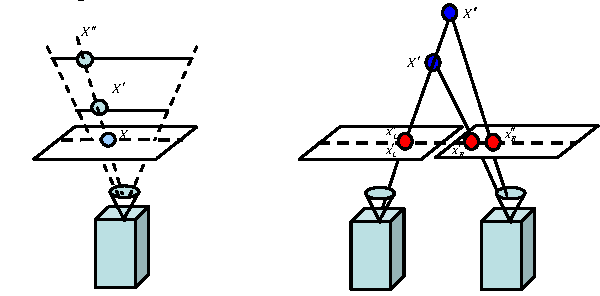
\includegraphics[width=0.5\linewidth]{Images/MonocularVsStereo.png}
            \caption{Monocular vs Stereo imaging}
        \end{figure}
        \textbf{Key Differences}\\\\
        \textbf{Number of Cameras:}
        \begin{itemize}
            \item Monocular: One camera.
            \item Stereo: Two cameras.
        \end{itemize}
        
        \textbf{\\Depth Information:}
        \begin{itemize}
            \item Monocular: Lacks direct depth perception; relies on computational methods to infer depth from visual cues over time or from known object sizes.
            \item Stereo: Provides direct depth information by analyzing the disparity between two simultaneous images.
        \end{itemize}
        
        \textbf{\\Complexity and Setup:}
        \begin{itemize}
            \item Monocular: Simpler setup, fewer components.
            \item Stereo: More complex setup, requires precise calibration and alignment of two cameras.
        \end{itemize}
        
        \textbf{\\Cost:}
        \begin{itemize}
            \item Monocular: Generally less expensive due to simpler hardware requirements.
            \item Stereo: More expensive due to additional hardware and computational requirements.
        \end{itemize}
    
        \textbf{\\Use Cases:}
        \begin{itemize}
            \item Monocular: Suitable for tasks where depth is less critical or can be inferred, such as in general photography or applications where other sensors can augment depth information.
            \item Stereo: Essential in scenarios where accurate real-time depth mapping is crucial, such as in augmented reality, precise 3D mapping, and autonomous vehicle navigation.
        \end{itemize}
        
        Understanding these differences is crucial when choosing between monocular and stereo vision systems for specific applications, as each has its strengths and limitations depending on the requirements of the task at hand.

    \section{Principles of Stereo Vision}
        \begin{itemize}
            \item \textbf{Binocular Disparity}\\
                The slight difference between the images seen by the left and right eyes is known as binocular disparity. This disparity arises because the two eyes are horizontally separated by a few centimeters (the interocular distance), which means each eye views the world from a slightly different angle.
                \begin{figure}[h]
                    \centering
                    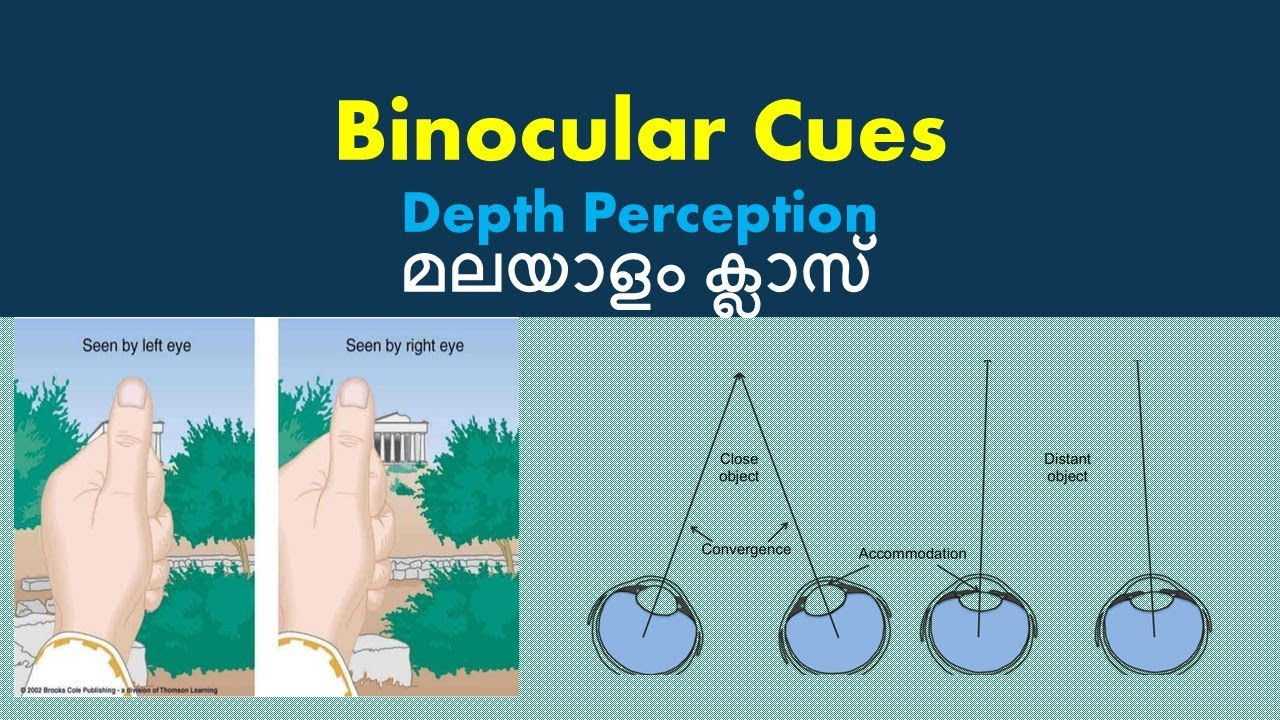
\includegraphics[width=0.5\linewidth]{Images/BinocularDisparity.jpg}
                    \caption{Binocular disparity}
                \end{figure}
                
            \item \textbf{Depth Perception}\\
                The brain uses the disparities between the two images to calculate distances to objects. Closer objects have greater disparity between the images than farther objects. This allows the brain to gauge depth and relative positions of objects in the environment.
                \begin{figure}[h]
                    \centering
                    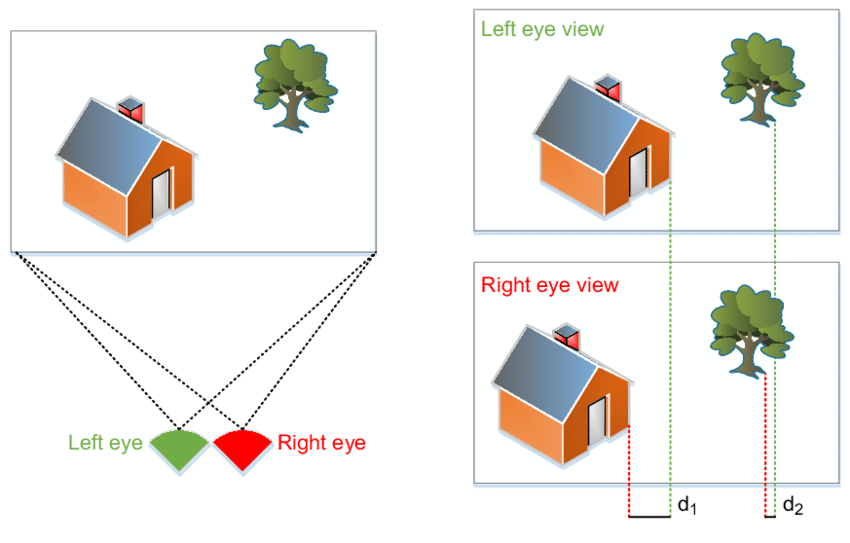
\includegraphics[width=0.5\linewidth]{Images/Depth-perception.png}
                    \caption{Depth perception}
                \end{figure}
                
            \item \textbf{Convergence}\\
                This is the inward movement of the eyes when focusing on an object that is close. The greater the convergence, the closer the object is perceived to be. So the convergence is the angle formed by your eyes and the observed object. The higher the angle value is, the nearer the observed object is to your eyes, and vice versa. The objects in front of the convergence point appears with pop-out effect and the objects behind the convergence point appears with deep-in effect.
                \begin{figure}[h]
                    \centering
                    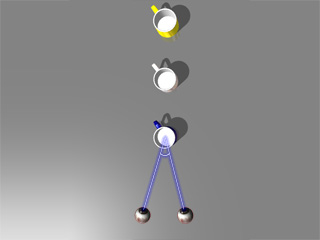
\includegraphics[width=0.25\linewidth]{Images/Convergence1.jpg}
                    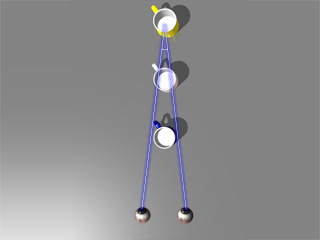
\includegraphics[width=0.25\linewidth]{Images/Convergence2.jpg}
                    \caption{Different convergence}
                    \label{fig:enter-label}
                \end{figure}
        \end{itemize}

    % \section{Fundamental Concept}
    %     \section{}
        
        

\chapter{What metrics are used for stereo vision?}
    Stereo vision can be divided into two problems: matching and 3D reconstruction. Out of
    these two, matching is considered to be the significant and complex problem. Matching is done to find corresponding points between stereo image pairs. Two image points $P_l$ in left image and $P_r$ in right image match if they result from the projection of the same point P in the scene, for example, $P_l$ and $P_r$ will have similar intensity or color. \\\\
    Stereo vision systems primarily focus on accurately determining the depth of objects from two slightly different viewpoints. The performance of such systems is typically evaluated using several key metrics. Here, we will explore some of these metrics, provide their formulas, and give numerical examples for each:
    
    \section{Disparity Error}
        Disparity refers to the difference in the location of the two corresponding points in their respective images \\
        \begin{center}
            \textbf{Disparity Error} = \(\left|d_{\text{true}} - d_{\text{estimated}} \right|\) \\
        \end{center}
        \begin{figure}[h]
            \centering
            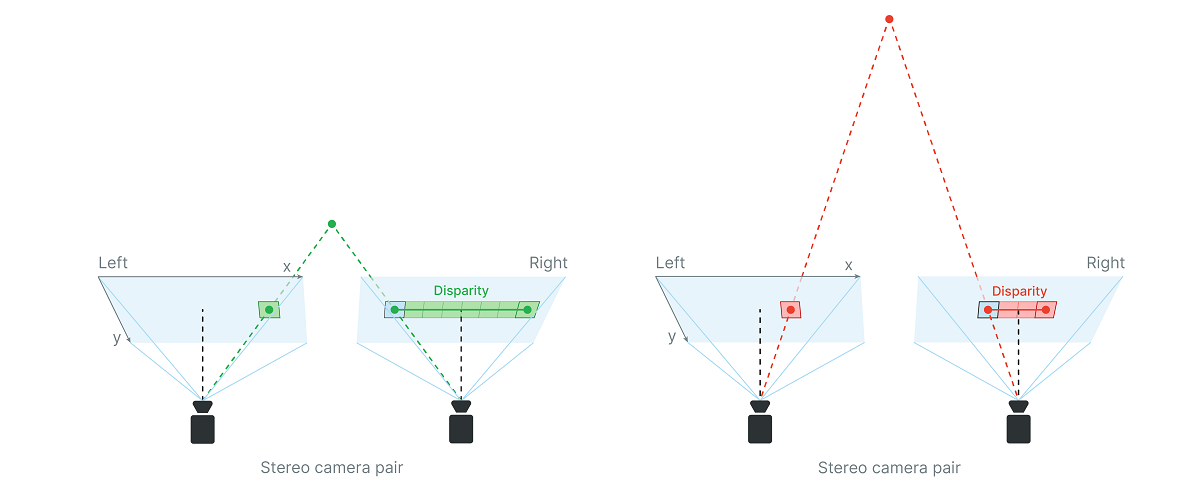
\includegraphics[width=0.5\linewidth]{Images/DisparityExplanation.png}
            \caption{Disparity error}
            \label{fig:enter-label}
        \end{figure}
        where \(d_{\text{true}}\) is the true disparity and \(d_{\text{estimated}}\) is the disparity estimated by the stereo vision algorithm.\\\\\\
        Relationship between the baseline(b), disparity(d), focal length(f) and depth(z):
        \begin{figure}[h]
            \centering
            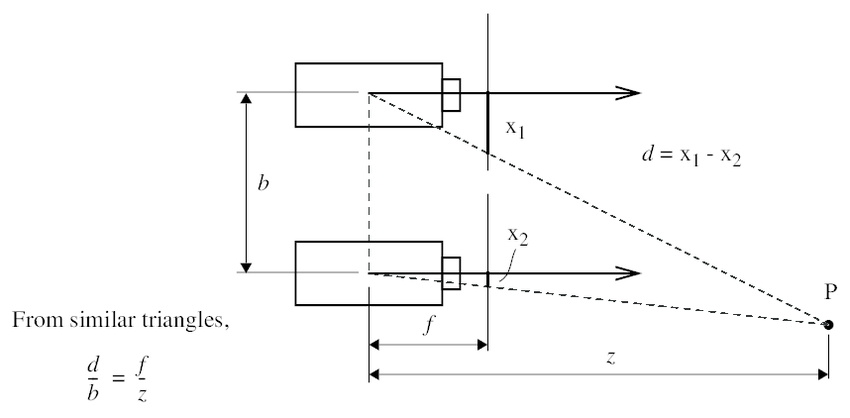
\includegraphics[width=0.5\linewidth]{Images/RelationBetweenbdfz.png}
            \caption{}
            \label{fig:enter-label}
        \end{figure}\\
        \textbf{Focal Lenght:}\\
        Focal length is the distance between the lens and the focal point, where the light rays converge or diverge. It is a critical parameter that determines the image quality and magnification of optical systems, including the human eye.
        \begin{figure}[h]
            \centering
            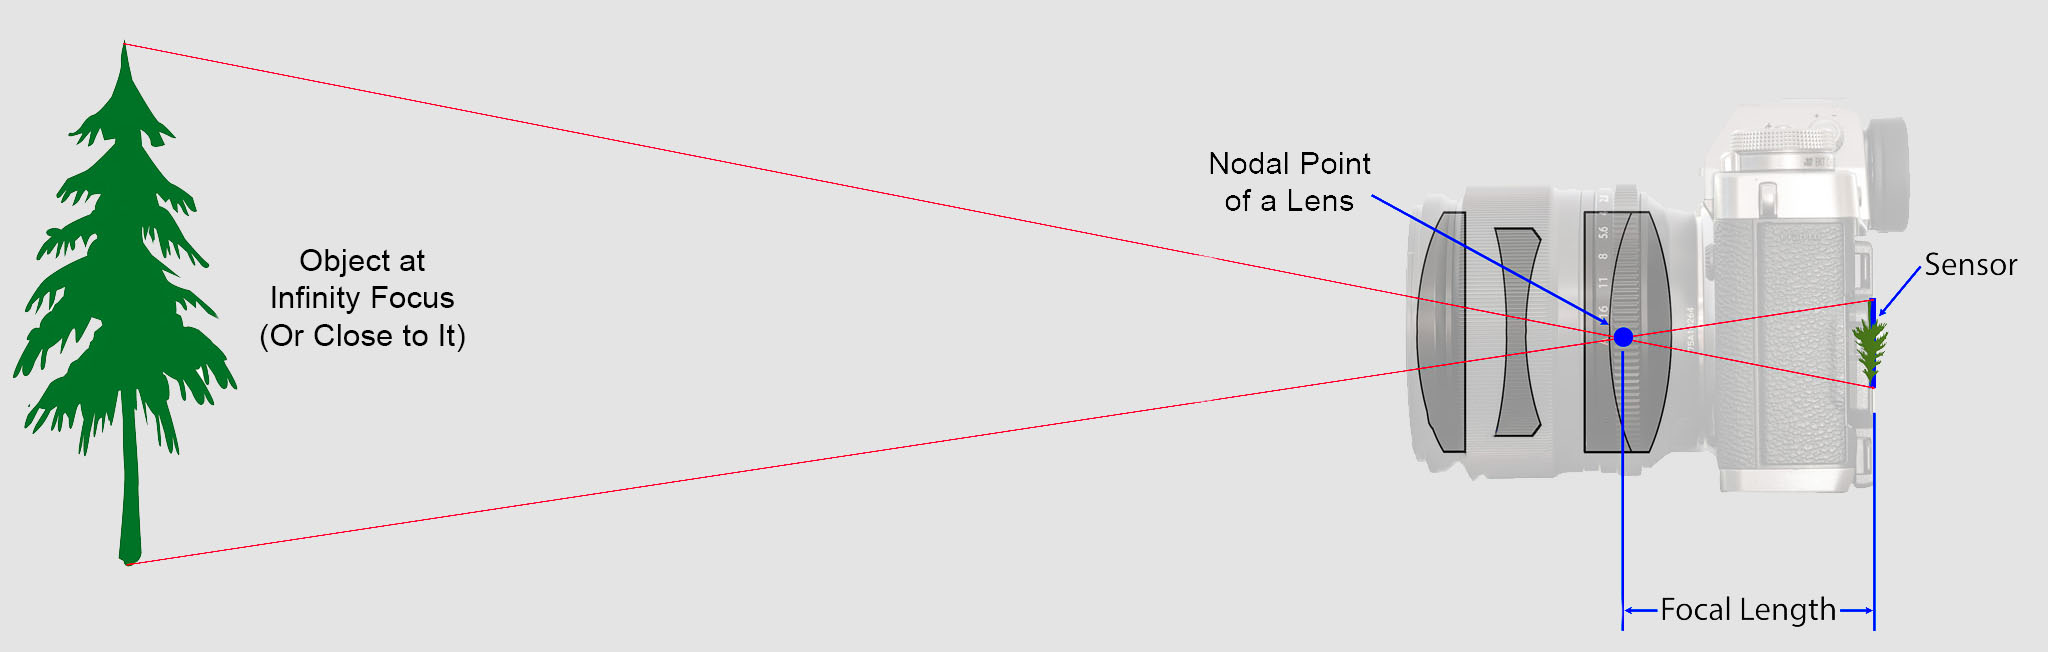
\includegraphics[width=0.5\linewidth]{Images/FocalLenght.jpg} 
            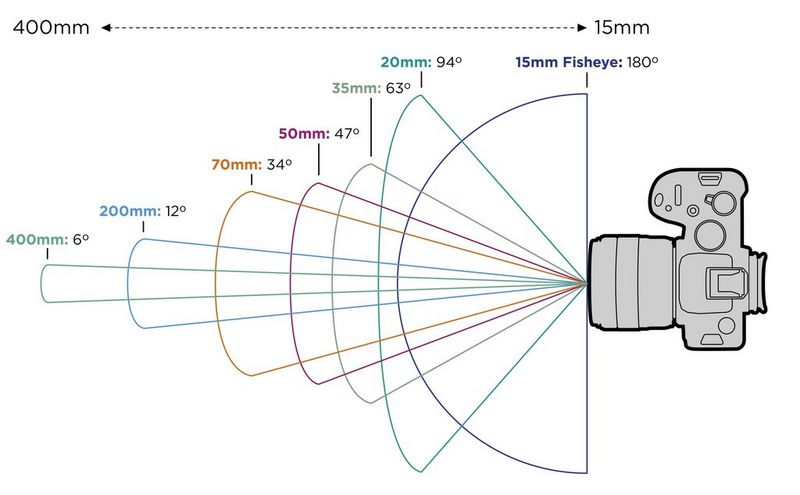
\includegraphics[width=0.5\linewidth]{Images/FocalLenghtOfCamera.jpg}
            \caption{Different focal lenght}
        \end{figure}\\
        \textbf{Field of view:}\\
        Field of view (FOV) is the open, observable area a person can see through their eyes or via an optical device, such as a camera. In the case of optical devices, FOV is the maximum area that the device can capture. In other words, it answers the question: "How much can the device see?"
        \begin{figure}[h]
            \centering
            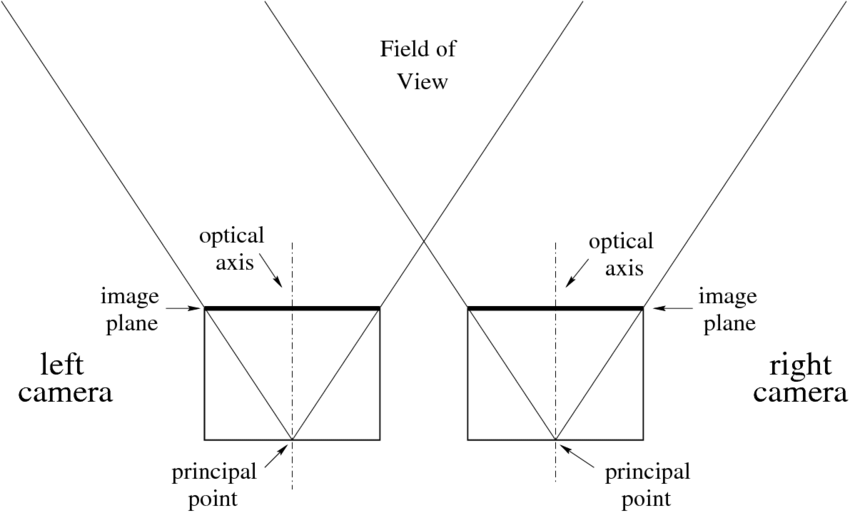
\includegraphics[width=0.5\linewidth]{Images/FieldOfView.png}
            \caption{Field of view}
            \label{fig:enter-label}
        \end{figure}
            
    
    \section{Depth Accuracy}
        Depth accuracy measures how close the computed depth is to the true depth of an object. It's directly related to the disparity error but translated into actual distance measurements.
        \begin{center}
            \text{Depth Accuracy} = \(\left| \frac{1}{d_{\text{estimated}}} - \frac{1}{d_{\text{true}}} \right| \times Bf\)
        \end{center}
        where \(B\) is the baseline (distance between the two cameras), \(f\) is the focal length of the cameras, and \(d\) is the disparity.\\ \\
        \begin{figure}
            \centering
            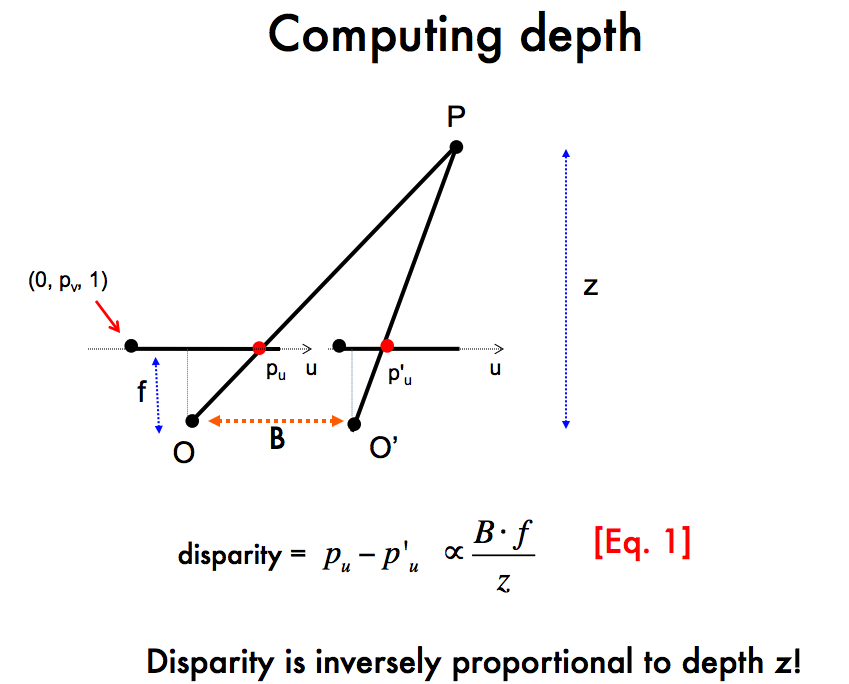
\includegraphics[width=0.5\linewidth]{Images/DepthAccuracy.png}
            \caption{Depth accuracy}
            \label{fig:enter-label}
        \end{figure}
    
    
    \section{Root Mean Square Error (RMSE) of Disparity}
        A quantitative approach is required to assess the performance of a stereo matching algorithm by estimating the quality of the final disparity map generated. The quality of the estimated disparity map is determined with
        respect to the ground truth by utilizing similarity measure Root Mean Square Error (RMSE). RMSE is computed in terms of disparity units between the resultant disparity map $d_{\text{estimated},i}$ and the ground truth map $d_{\text{true},i}$, which is the reference disparity map of the image. RMSE is given as follows:
        \[
        \text{RMSE} = \frac{1}{N} \sum_{i=1}^{N} \left|d_{\text{true},i} - d_{\text{estimated},i}\right|^2
        \]
        where \(N\) is the number of disparity measurements.\\\\
        \textbf{Disparity Map:}\\
        Given a pair of stereo images, to compute the disparity map, we first match every pixel in the left image with its corresponding pixel in the right image. Then we compute the distance for each pair of matching pixels. Finally, the disparity map is obtained by representing such distance values as an intensity image.
        Let’s consider, as an example, the following pair of stereo images and the corresponding disparity map.
        \begin{figure}[h]
            \centering
            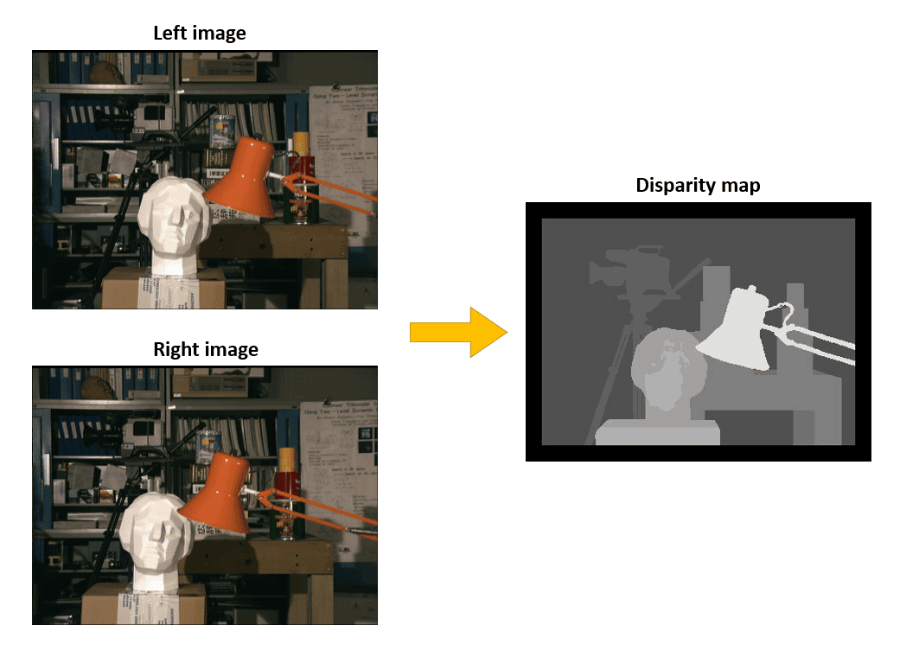
\includegraphics[width=0.5\linewidth]{Images/DisparityMap.png}
            \caption{Disparity map}
        \end{figure}\\
        We can see that the objects in the foreground, i.e., the lamp and the statue, appear fairly shifted in the stereo images, and therefore they are marked with brighter pixels in the disparity map. Conversely, the objects in the background have low disparity since their displacement in the stereo images is very small.\\\\
        As previously observed, the depth is inversely proportional to the disparity. If we know the geometric arrangement of the cameras, then the disparity map can be converted into a depth map using triangulation.\\\\
        When disparity is near zero, small disparity differences produce large depth differences. However, when disparity is large, small disparity differences do not change the depth significantly. Hence, stereo vision systems have high depth resolution only for objects relatively near the camera.\\\\        \href{https://www.researchgate.net/publication/281994923_Census_and_Segmentation-Based_Disparity_Estimation_Algorithm_Using_Region_Merging}{[*]Census and Segmentation-Based Disparity Estimation Algorithm Using Region Merging}
        
    \section{Percentage of Bad Matching Pixels (BMP)}
        This metric evaluates the percentage of pixels whose disparity error exceeds a certain threshold (e.g., 1 pixel).
        These metrics help in quantifying the performance of stereo vision systems and are essential for optimizing and comparing different algorithms. Each metric focuses on a different aspect of the disparity estimation process, providing a comprehensive evaluation of the system's accuracy and reliability.
        \[
        \text{BMP} = \left( \frac{\text{Number of bad matches}}{\text{Total number of matches}} \right) \times 100\%
        \]\\
        \href{https://www.researchgate.net/publication/365655310_Stereo_Image_Matching_Using_Adaptive_Morphological_Correlation}{[*]Stereo Image Matching Using Adaptive Morphological Correlation}


%%%%%%%%%%%%%%%%%%%%%%%%%%%%%%%%%%%%%%%%%%%%%%%%%%%%%%%%%%%%
\chapter{Methods and algorithm}
    \section{chronological list}
        Stereo vision has been a field of active research for many decades, resulting in a variety of methods that have evolved over time. Here’s a chronological list of some prominent methods and algorithms used for stereo vision, along with their approximate time of introduction:\\\\
        1980s\\
        \textbf{Block Matching Algorithm (BMA):} One of the earliest and simplest techniques, using fixed-size blocks to find correspondences based on similarity metrics like Sum of Absolute Differences (SAD).\\\\
        1990s\\
        \textbf{Dynamic Programming:} Introduced in the early 1990s, this method optimizes a cost function along horizontal scan-lines of the images.\\
        \textbf{Graph Cuts:} Late 1990s, this method models the stereo matching problem as a graph and finds the minimum cut that corresponds to the optimal disparity map.\\\\
        Early 2000s\\
        \textbf{Semi-Global Matching (SGM):} Introduced by Heiko Hirschmüller in 2005, SGM approximates a global optimization problem by combining multiple 1D optimizations and is known for its good balance between accuracy and computational efficiency.\\
        \textbf{Belief Propagation:} Early 2000s, this method uses probabilistic graphical models to infer disparities by message passing in a graphical structure.\\\\
        Mid to Late 2000s\\
        \textbf{PatchMatch Stereo:} An adaptation of the PatchMatch algorithm for stereo vision, introduced in 2009, which randomly searches for matching patches between images and refines the estimates iteratively.\\\\
        2010s\\
        Deep Learning-Based Methods; The rise of deep learning has significantly impacted stereo vision:\\
        \textbf{2014 - MC-CNN (Matching Cost with Convolutional Neural Network):} Introduced by Jure Žbontar and Yann LeCun, this method uses a CNN to learn a similarity measure for pairs of image patches.\\
        \textbf{2016 - DispNet:} A deep convolutional neural network trained end-to-end for disparity estimation.\\
        \textbf{2017 - GC-Net (Geometry and Context Network):} Integrates geometric priors and context information into a neural network for disparity estimation.\\\\
        2020s\\
        \textbf{RAFT-Stereo:} Building on the RAFT (Recurrent All-Pairs Field Transforms) method used for optical flow, adapted for stereo disparity prediction.\\
        \textbf{LEAStereo:} A lightweight and efficient architecture for stereo matching using neural networks, focusing on reducing computational costs while maintaining high accuracy.\\\\

    \section{Correspondence Problem}
        To compute the disparity map, we must address the so-called correspondence problem. This task aims at determining the pair of pixels in the stereo images that are projections of the same physical point in space.
        An important simplification of the problem can be obtained by the \textbf{rectification} of the stereo images. After this transformation, the corresponding points will lie on the same horizontal line. This reduces the 2D stereo correspondence problem to a 1D problem.
        The image rectification process is illustrated in the following figure:
        \begin{center}
            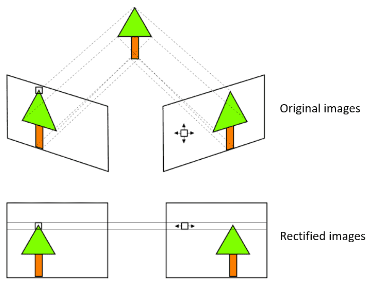
\includegraphics[width=0.5\linewidth]{Images/Rectification.png}
        \end{center}
        Two main problems:
        \begin{enumerate}
            \item Need to know focal length f, baseline b using prior knowledge or camera calibration
            \item Need to find corresponding point (xr,yr) for each (xl,yl) $\Rightarrow$ Correspondence problem
        \end{enumerate}        
    \section{Block Matching Algorithm (BMA)}
        A basic approach for finding corresponding pixels in stereo images is the \textbf{Block Matching algorithm}. It is based on comparing a small window around a point in the first image with multiple small blocks along the same horizontal line in the second image. For each pair of windows, a loss function is computed. The point $(\hat{x}$, $\hat{y})$ in the second image with minimum loss value is the best match for the point $(x, y)$ in the first image. Hence, the disparity value at the coordinate $(x, y)$ will be defined as:

        \[
        d(x, y) = (\hat{x} - x)
        \]

        \begin{figure}[h]
            \centering
            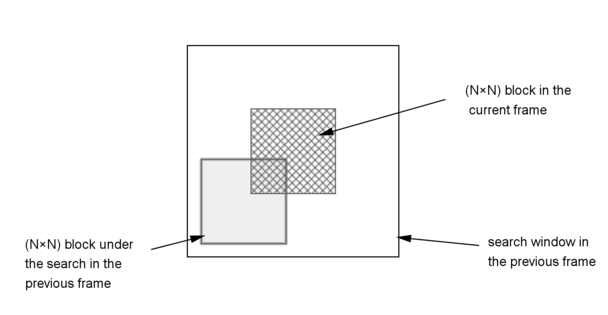
\includegraphics[width=0.5\linewidth]{Images/Block-matching_algorithm.png}
            \caption{BMA}
        \end{figure}
                
        \subsection{Sum of Absolute Differences (SAD)}
        
        Two different functions are usually used for finding the matching pixels. The first is the \textbf{Sum of Absolute Differences (SAD)}, which computes the sum of elementwise absolute differences of two windows \(W_L\) and \(W_R\), of size \(M \times N\), extracted from the two stereo images:
        
        \[
        SAD(W_L, W_R) = \sum_{i=1}^{M} \sum_{j=1}^{N} |W_L(i,j) - W_R(i,j)|
        \]
        
        This method is effective for quantifying the similarity between the two windows, where a lower SAD value indicates a better match.


        \subsection{Sum of Squared Differences (SSD)}
        The second function used is the Sum of Squared Differences (SSD), which calculates the sum of the squares of the differences:
        \[
        SSD(W_L, W_R) = \sum_{i=1}^N \sum_{j=1}^M (W_L^{ij} - W_R^{ij})^2
        \]
        \textbf{Comparison:}
        In general, SAD is preferable to SSD since it is faster and more robust to noise and outliers.\\\\
        \begin{figure}[h]
            \centering
            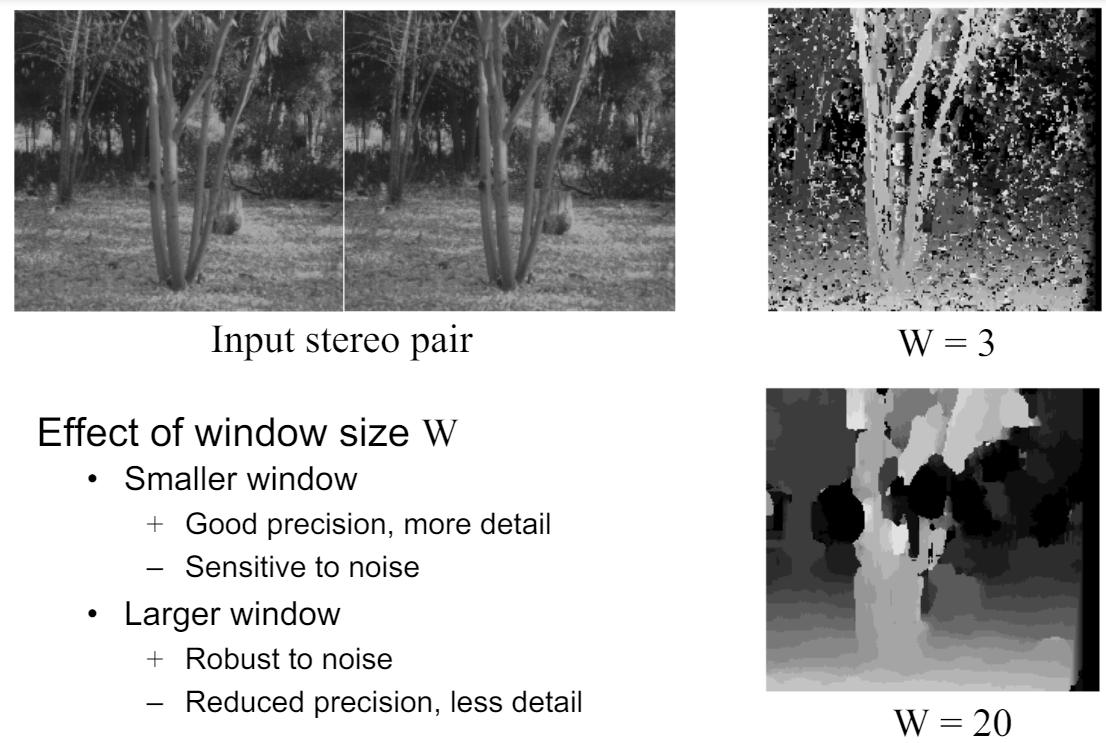
\includegraphics[width=0.5\linewidth]{Images/Window.png}
            \caption{ٍEffect of window size}
            % \label{fig:enter-label}
        \end{figure}
        \\\\\href{https://www.sciencedirect.com/science/article/pii/S235291481730045X}{[*]Survey of using GPU CUDA programming model in medical image analysis}\\
        \href{https://www.baeldung.com/cs/disparity-map-stereo-vision}{[*]Disparity Map in Stereo Vision}

        
    \section{Semi-Global Matching (SGM)}
        Semi-Global Matching (SGM),Developed by Heiko Hirschmüller in 2005, is particularly noted for its effectiveness in producing high-quality disparity maps with a relatively efficient computational cost. The method strikes a balance between local methods, which are fast but less accurate, and global methods, which are accurate but computationally expensive.\\
        SGM is based on the concept of approximating a global 2D optimization problem by aggregating multiple 1D constraints. The algorithm minimizes a cost function that is defined over the entire image, making it more robust to noise and occlusions compared to purely local methods.
        \subsection{Graphical Structure}
            SGM operates on a grid that corresponds to the image pixels, where each pixel is a node connected to its neighbors. The key idea is to perform cost aggregation along several paths through the image. Typically, SGM uses 8 or 16 paths covering different directions (e.g., horizontal, vertical, and diagonal) to integrate global context into the local matching costs.
        \subsection{Fundamental Steps and Formulas}
            \begin{enumerate}
                \item Cost Computation:
                 For each pixel and each possible disparity value, a matching cost is computed. Commonly used cost metrics include Sum of Absolute Differences (SAD), Sum of Squared Differences (SSD), or more sophisticated measures derived from mutual information or machine learning-based approaches.
                
              \begin{left}
               \textbf{ Matching Cost}:\\
                \(C(p,d)\) \\
                where \( C \) is the cost of assigning disparity \( d \) to pixel \( p \).
              \end{left}
                \item Cost Aggregation:
                The costs are aggregated along several paths through the image. For each pixel \( p \), the aggregated cost \( S \) for disparity \( d \) along a path \( r \) is computed by accumulating costs along that path, considering both the current cost and a smoothness penalty for disparity changes.
                 Aggregated Cost:
                 The costs are aggregated along several paths through the image. For each pixel \( p \), the aggregated cost \( S \) for disparity \( d \) along a path \( r \) is computed by accumulating costs along that path, considering both the current cost and a smoothness penalty for disparity changes.
                 \[ S(p,d) = C(p,d) + \min \left( S(p-r,d), \ S(p-r,d-1) + P_1, \ S(p-r,d+1) + P_1, \ \min_i S(p-r,i) + P_2 \right) - \min_i S(p-r,i) \]
                 Here, \( P_1 \) and \( P_2 \) are penalties for disparity changes: \( P_1 \) for small changes and \( P_2 \) for larger changes. The subtraction of \( \min_i S(p-r,i) \) ensures that the path costs do not grow unbounded.
                
                
                \item Disparity Selection:
                 After aggregation, the disparity for each pixel is determined by selecting the disparity that has the minimum aggregated cost over all paths.
                
                \[ D(p) = \arg\min_d \left( \sum_{\text{all paths } r} S(p,d) \right) \]
            \end{enumerate}
        \subsection{Loss Function Formula}
             The loss function in SGM combines data and smoothness terms to find the optimal disparity map by minimizing an energy function. The energy function 
            \( E(D) \)
            \( E(D) \) can be expressed as:
            \[ E(D) = \sum_p \left( C(p,D_p) + \sum_{q \in N(p)} P_1 \cdot 1[|D_p - D_q| = 1] + P_2 \cdot 1[|D_p - D_q| > 1] \right) \] where:
            \begin{itemize}
                \item \( p \) and \( q \) are pixel positions.
                \item \\ \( D_p \) is the disparity at pixel \( p \).
                \item \\ \( C(p, D_p) \) is the matching cost for pixel \( p \) at disparity \( D_p \).
                \item \\ \( N(p) \) is the set of neighboring pixels of \( p \).
                \item \\ \( P_1 \) is a penalty for small disparity changes (e.g., 1 pixel).
                \item \\ \( P_2 \) is a larger penalty for larger disparity changes.
            \end{itemize}
            \vspace{10}
            Consider a 3x3 image patch with the following pixel intensities: \begin{verbatim}
    Image A:
    10 20 30
    40 50 60
    70 80 90
    
    Image B (shifted by 1 pixel to the right):
    0 10 20
    0 40 50
    0 70 80
    \end{verbatim}
 \\ Assume we are computing the disparity for the pixel at position (2, 2) in Image A (intensity 50). We compare it with various disparities \(D\):
            \begin{enumerate}
                \item  Matching Cost \(C(p, D_p)\): \begin{itemize} \item For \(D = 0\): \(C(2, 2, 0) = |50 - 50| = 0\) \item For \(D = 1\): \(C(2, 2, 1) = |50 - 40| = 10\) \item For \(D = 2\): \(C(2, 2, 2) = |50 - 0| = 50\) \end{itemize}
                \item Smoothness Terms: \begin{itemize} \item Assume \(P_1 = 1\) and \(P_2 = 10\). \end{itemize}
                \item Energy Calculation:\\ \vspace{15} 
                     For \( D = 0 \): \[ E(0) = C(2,2,0) + \sum_{q \in N(2,2)} \left( P_1 \cdot 1[|D_{(2,2)} - D_q| = 1] + P_2 \cdot 1[|D_{(2,2)} - D_q| > 1] \right) \]
                    Assume neighboring disparities \( D_q \) are all 0 (initial guess):
                     \[ E(0) = 0 + 0 = 0 \] \\
                     For \( D = 1 \):
                        \[
                        E(1) = C(2, 2, 1) + \sum_{q \in N(2,2)} \left( P_1 \cdot 1[|1 - D_q| = 1] + P_2 \cdot 1[|1 - D_q| > 1] \right)
                        \]
                        
                        Assuming \( D_q \) are all 0:
                        
                        \[
                        E(1) = 10 + 4 \cdot P_1 = 10 + 4 \cdot 1 = 14
                        \]
                        
                        For \( D = 2 \):
                        
                        \[
                        E(2) = C(2, 2, 2) + \sum_{q \in N(2,2)} \left( P_1 \cdot 1[|2 - D_q| = 1] + P_2 \cdot 1[|2 - D_q| > 1] \right)
                        \]
                        
                        Assuming \( D_q \) are all 0:
                        
                        \[
                        E(2) = 50 + 4 \cdot P_2 = 50 + 4 \cdot 10 = 90
                        \]

            \end{enumerate}
%%%%%%%%%%%%%%%%%%%%%%%%%%%%%%%%%%%%%%%%%%%%%%%%%%%%%%%%%%%%%%%%%%%%%%%%%%%%%%%%%%%%%%%%%%%%%%%%%%%%%%%%%%%%%%%%%%%%%%%%%%%%%%%%%%%%%%%%%%%%%%%%%%%%%%%%%%%%%%%%%%%%%%%%%%%%%%%%%%%%%%%%%%%%%%%%%%%%%%%%%%%%%%%%%%%%%%%%%%%%%%%%%%%%%%%%%%%%%%%%%%%%%%%%%%%%%%%%%%%%%%%%%%%%%%%%%%%%%%%%%%%%%%%%%%%%%%%%%%%%%%%%%%%%%%%%%%%%%%%%%%%%%%%

\section{PatchMatch Stereo}
PatchMatch Stereo is an efficient stereo matching algorithm that extends the PatchMatch algorithm originally developed for image editing tasks. The PatchMatch Stereo algorithm aims to find correspondences between patches in two stereo images to construct a disparity map. This disparity map indicates the differences in the position of objects as seen from the two viewpoints, which can be used to infer depth information.\\
\subsection{Graphical Structure}
The core idea of PatchMatch Stereo lies in its random initialization and iterative refinement process. The algorithm operates on two main images:\\
\begin{itemize}
    \item Left Image (Reference Image)
    \item Right Image (Target Image)
\end{itemize}
Both images are segmented into patches (small blocks or windows of pixels). The goal is to find for each patch in the left image the best matching patch in the right image along the same scanline (assuming rectified stereo images where corresponding points are on the same horizontal line).

\vspace{20}
\subsection{PatchMatch Stereo Algorithm}
\
The PatchMatch Stereo algorithm involves the following steps:
\begin{enumerate}
    \item \textbf{Initialization:} \\
Each patch in the left image is randomly assigned a disparity value (i.e., the horizontal shift required to find the corresponding patch in the right image).
    \item \textbf{Propagation:} \\
    The algorithm iteratively updates the disparity values by propagating good matches from neighboring patches. This is based on the assumption that neighboring points in an image are likely to have similar disparity values. The propagation occurs in alternating scan directions (left-to-right, right-to-left) to ensure consistency and to propagate good estimates across the image.
    \item \textbf{Random Search:} \\
    After propagation, the algorithm refines the disparity estimates by randomly searching around the current best estimate. This random search is performed in exponentially decreasing windows to converge to the best match.
    
\end{enumerate}
\vspace{15}
\subsection{Mathematical Formulation}
The similarity between two patches centered at pixel \( p \) in the left image and pixel \( p' \) in the right image is typically measured using a cost function such as Sum of Absolute Differences (SAD), Sum of Squared Differences (SSD), or normalized cross-correlation. The disparity \( d \) at pixel \( p \) is adjusted to minimize this cost: \[ C(p,d) = \sum_{(x,y) \in \text{patch}} |I_L(x,y) - I_R(x-d,y)| \] Where: \( I_L \) is the intensity of the left image. \\ \( I_R \) is the intensity of the right image. \\ \( (x,y) \) are the coordinates within the patch centered around pixel \( p \).
\vspace{15}
\subsection{\textbf{Iterative Refinement:}}
The disparity for each patch is updated based on the lowest cost calculated during the propagation and random search stages: Propagation: Check disparities from neighboring patches (e.g., left and above in left-to-right pass). Random Search: Adjust the disparity by random offsets and evaluate the cost, focusing on smaller ranges in subsequent iterations. \\ \\
- Consider a simple scenario with a left image and a right image each containing distinct blocks or patterns. Suppose the initial disparities are randomly assigned. During propagation, if a nearby patch has a good disparity estimate (i.e., low matching cost), this estimate is tested for the current patch. If it results in a lower cost than the current disparity, it is adopted. During the random search phase, this disparity might be randomly adjusted within a shrinking window to refine the match further.
PatchMatch Stereo is particularly effective due to its ability to quickly converge to good disparity estimates through its random initialization and iterative refinement, leveraging both local coherence and global optimization strategies. This makes it suitable for large-scale and real-time stereo vision applications.
%%%%%%%%%%%%%%%%%%%%%%%%%%%%%%%%%%%%%%%%%%%%%%%%%%%%%%%%%%%%%%%%%%%%%%%%%%%%%%%%%%%%%%%%%%%%%%%%%%%%%%%%%%%%%%%%%%%%%%%%%%%%%%%%%%%%%%%%%%%%%%%%%%%%%%%%%%%%%%%%%%%%%%%%%%%%%%%%%%%%%%%%%%%%%%%%%%%%%%%%%%%%%%%%%%%%%%%%%%%%%%%%%%%%%%%%%%%%%%%%%%%%%%%%%%%%%%%%%%

In stereo vision algorithms like PatchMatch Stereo, the primary goal is to determine the disparity between corresponding points in a stereo pair of images, which can be used to compute depth. A loss function is used to measure the quality of matching between patches in the left and right images. One common loss function is the Sum of Absolute Differences (SAD), though others like Sum of Squared Differences (SSD) can also be used.\\
\subsection{Loss Function Formula}
For the Sum of Absolute Differences (SAD), the loss function for a patch centered at pixel \( p \) in the left image with disparity \( d \) is defined as:

\[
SAD(p,d) = \sum_{(x,y) \in \text{patch}} |I_L(x,y) - I_R(x-d,y)|
\]

Where:

\begin{itemize}
    \item \( I_L \) is the intensity of the left image. \\
    \item \( I_R \) is the intensity of the right image. \\
    \item \( (x,y) \) are the coordinates of pixels within the patch centered at \( p \). \\
    \item \( d \) is the disparity value.
\end{itemize}
-\textbf{Numerical Example} \\

Let's consider a simple numerical example with small 3x3 patches to illustrate how the loss function operates:

Assume the following intensity values for a patch in the left and right images with different disparities:
\begin{enumerate}
\item Left Image Patch at position \((3,3)\): \\
\[
\begin{array}{ccc}
100 & 110 & 120 \\
130 & 140 & 150 \\
160 & 170 & 180 \\
\end{array}
\]
\item Right Image Patches at position \((3-d,3)\) for disparities \( d=1 \) and \( d=2 \):
\begin{enumerate}
    

\item For \( d=1 \) (Shift right by 1 pixel):
\[
\begin{array}{ccc}
105 & 115 & 125 \\
135 & 145 & 155 \\
165 & 175 & 185 \\
\end{array}
\]

\item For \( d=2 \) (Shift right by 2 pixels):
\[
\begin{array}{ccc}
108 & 118 & 128 \\
138 & 148 & 158 \\
168 & 178 & 188 \\
\end{array}
\]
\end{enumerate}
\end{enumerate}

\textbf{Calculate SAD for both disparities:} \\

\begin{itemize}
    \item \textbf{SAD for \( d=1 \):}

\[
\begin{aligned}
SAD(d=1) &= |100 - 105| + |110 - 115| + |120 - 125| \\
         &\quad + |130 - 135| + |140 - 145| + |150 - 155| \\
         &\quad + |160 - 165| + |170 - 175| + |180 - 185| \\
         &= 5 + 5 + 5 + 5 + 5 + 5 + 5 + 5 + 5 \\
         &= 45
\end{aligned}
\]
    
    \item \textbf{SAD for \( d=2 \):}
    \[
\begin{aligned}
SAD(d=2) &= |100 - 108| + |110 - 118| + |120 - 128| \\
         &\quad + |130 - 138| + |140 - 148| + |150 - 158| \\
         &\quad + |160 - 168| + |170 - 178| + |180 - 188| \\
         &= 8 + 8 + 8 + 8 + 8 + 8 + 8 + 8 + 8 \\
         &= 72
\end{aligned}
\]
\end{itemize}
\vspace{15}
From this calculation, \( d=1 \) yields a lower SAD value of 45 compared to \( d=2 \) with a SAD value of 72. Thus, for this patch, a disparity of 1 provides a better match between the left and right images than a disparity of 2.\\

This kind of calculation is performed for each patch across the image, and the disparity that minimizes the loss function for each patch is chosen as the best estimate. This process is iteratively refined using PatchMatch Stereo's propagation and random search mechanisms.

%%%%%%%%%%%%%%%%%%%%%%%%%%%%%%%%%%%%%%%%%%%%%%%%%%%%%%%%%%%%%%%%%%%%%%%%%%%%%%%%%%%%%%%%%%%%%%%%%%%%%%%%%%%%%%%%%%%%%%%%%%%%%%%%%%%%%%%%%%%%%%%%%%%%%%%%%%%%%%%%%%%%%%%%%%%%%%%%%%%%%%%%%%%%%%%%%%%%%%%%%%%%%%%%%%%%%%%%%%%%%%%%%%%%%%%%%%%%%%%%%%%%%%%%%%%%%%%%%%

\section{MC-CNN}
MC-CNN (Matching Cost with Convolutional Neural Network) is an approach that uses deep learning to compute the similarity between image patches in stereo vision tasks. This method was introduced to improve the accuracy and robustness of disparity estimation by learning a function that can better discriminate between similar and dissimilar patches compared to traditional hand-crafted measures like Sum of Absolute Differences (SAD) or Sum of Squared Differences (SSD).\\
\vspace{8}
\subsection{Graphical Structure of MC-CNN}
The MC-CNN architecture typically consists of two main components:
\begin{enumerate}
    \item \textbf{Siamese Network Architecture:} This structure involves two convolutional neural networks (CNNs) that share weights. Each network processes one of the stereo images (left or right). The goal is to extract feature vectors from corresponding patches in both images.
    \item \textbf{Matching Cost Computation:} After feature extraction, the similarity between the feature vectors of corresponding patches is computed to generate a matching cost. This can be done using various methods, like calculating the L1 distance, L2 distance, or by feeding the concatenated or difference of features into additional network layers that output a scalar matching cost.
\end{enumerate}
\vspace{15}

-Here’s a simple visualization of the MC-CNN structure: \\
\begin{center}
    \begin{tikzpicture}[auto, node distance=2cm,>=latex']
    % Nodes
    \node [input, name=inputL] {Left Image Patch};
    \node [block, right of=inputL, node distance=3cm] (cnnL) {CNN};
    \node [input, below of=inputL, node distance=2cm] (inputR) {Right Image Patch};
    \node [block, right of=inputR, node distance=3cm] (cnnR) {CNN};
    \node [block, right of=cnnL, node distance=4cm] (cost) {Cost Computation};
    \node [output, right of=cost, node distance=4cm] (matching) {Matching Cost};

    % Paths
    \draw [->] (inputL) -- (cnnL);
    \draw [->] (inputR) -- (cnnR);
    \draw [->] (cnnL) -- ++(1.5,0) |- (cost);
    \draw [->] (cnnR) -- ++(1.5,0) |- (cost);
    \draw [->] (cost) -- (matching);
    
    % Labels
    \node [above of=cnnL, node distance=1cm] {};
    \node [above of=cnnR, node distance=1cm] {};

\end{tikzpicture}
\end{center}
\vspace{25}
\subsection{Mathematical Representation} \\ \\
The mathematical formulation of the MC-CNN involves several key components:
\begin{enumerate}
    \item Feature Extraction: \\
    Let \( f(I_L, p) \) and \( f(I_R, p') \) denote the feature vectors extracted by the CNNs from patches centered at pixel \( p \) in the left image \( I_L \) and pixel \( p' \) in the right image \( I_R \), respectively.
    \item Matching Cost Calculation:\\
    Let \( f(I_L, p) \) and \( f(I_R, p') \) denote the feature vectors extracted by the CNNs from patches centered at pixel \( p \) in the left image \( I_L \) and pixel \( p' \) in the right image \( I_R \), respectively.
    The matching cost \( C(p, p') \) between the patches at \( p \) and \( p' \) is computed based on their feature vectors. A common choice is the Euclidean distance:
    \[
    C(p, p') = \| f(I_L, p) - f(I_R, p') \|
    \]
    
    Alternatively, the matching cost could be computed using a learned function:
    \[
    C(p, p') = g(f(I_L, p), f(I_R, p'))
    \]
    
    where \( g \) is a function (possibly another neural network) that takes the feature vectors (or their concatenation, or element-wise difference) and outputs a scalar cost.
\end{enumerate}

\subsection{Training the Network}
The MC-CNN is typically trained using a dataset of stereo image pairs with known disparity values. The training process involves minimizing a loss function that encourages the network to produce low costs for correct matches (patches with the correct disparity) and high costs for incorrect matches. Commonly used loss functions include contrastive loss, hinge loss, or log-likelihood loss, depending on the specific formulation of the matching cost.
\vspace{15}
\subsection*{Example Application:}
In practice, once the network is trained, for each pixel in the left image, the algorithm computes the matching costs for a range of disparities (possible shifts to the right image). The disparity that minimizes this cost is selected as the estimated disparity for that pixel, forming the disparity map of the scene.
\\
MC-CNN represents a significant step forward in stereo matching technology because it leverages the powerful feature extraction capabilities of CNNs, allowing it to outperform traditional methods, particularly in challenging conditions such as low-texture areas, repetitive patterns, or lighting variations.

%%%%%%%%%%%%%%%%%%%%%%%%%%%%%%%%%%%%%%%%%%%%%%%%%%%%%%%%%%%%%%%%%%%%%%%%%%%%%%%%%%%%%%%%%%%%%%%%%%%%%%%%%%%%%%%%%%%%%%%%%%%%%%%%%%%%%%%%%%%%%%%%%%%%%%%%%%%%%%%%%%%%%%%%%%%%%%%%%%%%%%%%%%%%%%%%%%%%%%%%%%%%%%%%%%%%%%%%%%%%%%%%%%%%%%%%%%%%%%%%%%%%%%%%%%%%%%%%%%
In the context of MC-CNN (Matching Cost with Convolutional Neural Networks) for stereo matching, the training process involves minimizing a loss function that accurately captures the differences between the predicted and true disparities. One commonly used loss function for this purpose is the \textbf{contrastive loss}, which is designed to ensure that similar pairs (correct matches) have a low distance in the feature space, and dissimilar pairs (incorrect matches) have a distance greater than a margin.\\
\subsection{Contrastive Loss Formula}
The contrastive loss for a pair of patches \( (p, p') \) from the left and right images respectively, with labels \( y \) indicating if they are a match (1 for match, 0 for non-match), can be expressed as:

\[
L(p, p', y) = y \cdot D^2 + (1 - y) \cdot \max(0, m - D)^2
\]
Where:
\begin{itemize}
    \item \( D \) is the Euclidean distance between the feature vectors extracted from the patches \( p \) and \( p' \), \( D = \| f(I_L, p) - f(I_R, p') \| \).
    \item \( m \) is a margin, a hyperparameter that defines how far the distances of non-matching pairs should be pushed apart.
    \item \( y \) is a binary label, where \( y = 1 \) if \( p \) and \( p' \) are a true match (same disparity), and \( y = 0 \) if they are not.
\end{itemize}
\vspace{20}
\subsection*{Numerical Example}
Let's consider a simplified example where the feature vectors extracted by the CNN for a certain patch from the left and right images are as follows:
\begin{itemize}
    \item Feature vector from left image patch \( f(I_L, p) = [1.0, 2.0] \)
    \item Feature vector from right image patch for a correct match \( f(I_R, p') = [1.1, 2.1] \)
    \item Feature vector from right image patch for an incorrect match \( f(I_R, p'') = [3.0, 4.0] \)
    \item Assume a margin \( m = 1.5 \).
\end{itemize}
\vspace{10}
\subsection*{Calculate the Euclidean distance for both cases:}
\begin{enumerate}
    \item \textbf{Correct match \( (p, p') \):} \\
            \[
            D = \| [1.0, 2.0] - [1.1, 2.1] \| = \sqrt{(1.0 - 1.1)^2 + (2.0 - 2.1)^2} = \sqrt{0.01 + 0.01} = \sqrt{0.02} \approx 0.141
            \]
    \item \textbf{Incorrect match \( (p, p'') \)}:\\
            \[
            D = \| [1.0, 2.0] - [3.0, 4.0] \| = \sqrt{(1.0 - 3.0)^2 + (2.0 - 4.0)^2} = \sqrt{4 + 4} = \sqrt{8} \approx 2.828
            \]
\end{enumerate}
\\
\subsection*{Apply the contrastive loss formula:}
\begin{enumerate}
    \item \textbf{Correct match \( (y = 1) \):} \\
         \[
            L(p, p', y = 1) = 1 \cdot (0.141)^2 + 0 \cdot \max(0, 1.5 - 0.141)^2 = 0.019921
            \]
            \\
     \item \textbf{Incorrect match \( (y = 0) \):}\\
            \[
            L(p, p'', y = 0) = 0 \cdot (2.828)^2 + 1 \cdot \max(0, 1.5 - 2.828)^2 = 0 \quad (\text{since } 1.5 - 2.828 < 0)
            \]
\end{enumerate}
\vspace{8}
Here, the loss for the correct match is quite low as expected, indicating a good prediction by the network, while the loss for the incorrect match is zero, as the distance exceeds the margin, showing that the network is effectively distinguishing between matching and non-matching patches.

%%%%%%%%%%%%%%%%%%%%%%%%%%%%%%%%%%%%%%%%%%%%%%%%%%%%%%%%%%%%%%%%%%%%%%%%%%%%%%%%%%%%%%%%%%%%%%%%%%%%%%%%%%%%%%%%%%%%%%%%%%%%%%%%%%%%%%%%%%%%%%%%%%%%%%%%%%%%%%%%%%%%%%%%%%%%%%%%%%%%%%%%%%%%%%%%%%%%%%%%%%%%%%%%%%%%%%%%%%%%%%%%%%%%%%%%%%%%%%%%%%%%%%%%%%%%%%%%%%

\section{DispNet}
DispNet is a deep learning architecture designed for the task of disparity estimation in stereo vision, which is crucial for applications such as autonomous driving and 3D reconstruction. The architecture is based on the principles of convolutional neural networks (CNNs) and is specifically tailored to generate dense pixel-wise disparity maps directly from stereo image pairs. \\
\subsection{Graphical Structure of DispNet}
DispNet typically follows an encoder-decoder architecture with skip connections, which is common in tasks that involve dense predictions like semantic segmentation or depth estimation. Its design includes several innovative elements to effectively handle the specifics of disparity estimation:
\begin{enumerate}
    \item \textbf{Input Layer:} The network takes a pair of stereo images (left and right images) as input. These images can be concatenated along the channel dimension, effectively treating the stereo pair as a multi-channel single input.
    \item \textbf{Encoder:} The encoder consists of a series of convolutional layers that progressively downsample the input, capturing increasingly abstract features at higher levels. This part of the network learns to encode important features from both images that are relevant for disparity estimation.
    \item \textbf{Decoder:} The decoder uses upsampling layers (often transposed convolutions) to progressively increase the spatial dimensions of the processed features. At each stage of the decoder, features from the corresponding encoder stage are often added or concatenated (via skip connections), helping to preserve high-resolution details necessary for pixel-wise disparity prediction.
    \item \textbf{Skip Connections:} These are crucial for combining low-level, fine-grained details with high-level semantic information, which enhances the network's ability to predict accurate disparities at pixel level.
    \item \textbf{Output Layer:} The final layer of the network typically consists of a convolutional layer that maps the high-dimensional feature data to a one-channel output image representing the disparity map.
\end{enumerate}
\vspace{10}
\subsection*{Diagram Overview}
Here's a simplified visualization of the DispNet architecture:
\begin{center}
   \large
    \begin{tikzpicture}[auto, node distance=2cm,>=latex']
    % Nodes
    \node [block] (input) {Input (Stereo Image Pair)};
    \node [block, below of=input, node distance=1.5cm] (conv1) {Convolutional Layers \\ (downsampling)};
    \node [block, below of=conv1, node distance=1.5cm] (encoder) {Encoder Feature Extraction};
    \node [block, below of=encoder, node distance=1.5cm] (conv2) {Convolutional Layers \\ (upsampling)};
    \node [block, below of=conv2, node distance=1.5cm] (skip) {Skip Connections from Encoder};
    \node [block, below of=skip, node distance=1.5cm] (final) {Final Convolution to produce Disparity Map};
    \node [block, below of=final, node distance=1.5cm] (output) {Output (Disparity Map)};

    % Paths
    \draw [->] (input) -- (conv1);
    \draw [->] (conv1) -- (encoder);
    \draw [->] (encoder) -- (conv2);
    \draw [->] (conv2) -- (skip);
    \draw [->] (skip) -- (final);
    \draw [->] (final) -- (output);

\end{tikzpicture}
\end{center}
\vspace{20}
\subsection{Mathematical Representation}
The disparity estimation can be formulated as a regression problem where the network learns a mapping function from the input stereo images to the disparity map. The typical loss function used is either an L1 or L2 loss between the predicted disparity map and the ground truth:
\\
\[
L = \frac{1}{N} \sum_{i=1}^{N} \left| D_{\text{pred}}(i) - D_{\text{true}}(i) \right|
\]
\\ or \\
\[
L = \frac{1}{N} \sum_{i=1}^{N} \left( D_{\text{pred}}(i) - D_{\text{true}}(i) \right)^2
\]

Where :
\begin{itemize}
    \item \( D_{\text{pred}} \) is the predicted disparity map. \\
    \item \( D_{\text{true}} \) is the ground truth disparity map. \\
    \item \( N \) is the total number of pixels in the disparity map.
\end{itemize}
\vspace{15}
\subsection{Training and Application}
During training, DispNet is usually trained end-to-end using a dataset of stereo images along with their corresponding ground truth disparity maps. The network learns to minimize the disparity prediction error across the training set, adjusting its weights accordingly.

Once trained, DispNet can generate disparity maps for new pairs of stereo images, which can then be used in various applications like 3D scene reconstruction, object detection in 3D space, and navigation assistance in autonomous vehicles.
\newpage
DispNet, as a deep learning model for disparity estimation, typically uses a loss function that directly measures the error between the predicted disparity map and the ground truth. Common choices for the loss function in disparity estimation tasks include the L1 loss (mean absolute error) and the L2 loss (mean squared error). The L1 loss is often preferred due to its robustness to outliers.\\
\subsection{L1 Loss Formula}
The L1 loss for disparity estimation can be formulated as:
\begin{center}
    \[
L(\theta) = \frac{1}{N} \sum_{i=1}^{N} \left| D_{\text{pred}}(i) - D_{\text{true}}(i) \right|
\]
\end{center}
where:
\begin{itemize}
    \item \(\theta\) represents the parameters of the network. \\
    \item \( D_{\text{pred}}(i) \) is the predicted disparity at pixel \( i \). \\
    \item \( D_{\text{true}}(i) \) is the ground truth disparity at pixel \( i \). \\
    \item \( N \) is the total number of pixels in the images.
\end{itemize}
\vspace{20}
\subsection*{Numerical Example}
Let's consider a simple example with a small disparity map of size 2x2 pixels. Assume the predicted disparities and the ground truth disparities for this small region are as follows:

    \textbf{Predicted Disparity Map}, \( D_{\text{pred}} \):
\[
        \begin{bmatrix}
        10 & 12 \\
        15 & 20 \\
        \end{bmatrix}
        \]
        
        \textbf{Ground Truth Disparity Map}, \( D_{\text{true}} \):
        \[
        \begin{bmatrix}
        12 & 11 \\
        14 & 22 \\
        \end{bmatrix}
        \]
\subsection*{Calculation of L1 Loss}
Calculate the absolute difference for each corresponding pixel, and then compute the average:
\begin{itemize}
    \item \textbf{Absolute Differences:}
            \[
            \begin{bmatrix}
            |10 - 12| & |12 - 11| \\
            |15 - 14| & |20 - 22| \\
            \end{bmatrix}
            =
            \begin{bmatrix}
            2 & 1 \\
            1 & 2 \\
            \end{bmatrix}
            \]
    \item \textbf{Sum of Absolute Differences:}
                \[
                2 + 1 + 1 + 2 = 6
                \]
    \item \textbf{Mean Absolute Error (L1 Loss):}
            \[
            L(\theta) = \frac{6}{4} = 1.5
            \]
\end{itemize}
\vspace{8}
In this example, the L1 loss is 1.5, indicating that, on average, each pixel's disparity error is 1.5 units away from the true disparity.

%%%%%%%%%%%%%%%%%%%%%%%%%%%%%%%%%%%%%%%%%%%%%%%%%%%%%%%%%%%%%%%%%%%%%%%%%%%%%%%%%%%%%%%%%%%%%%%%%%%%%%%%%%%%%%%%%%%%%%%%%%%%%%%%%%%%%%%%%%%%%%%%%%%%%%%%%%%%%%%%%%%%%%%%%%%%%%%%%%%%%%%%%%%%%%%%%%%%%%%%%%%%%%%%%%%%%%%%%%%%%%%%%%%%%%%%%%%%%%%%%%%%%%%%%%%%%%%%%%
\section{GC-Net}
GC-Net, or Geometry and Context Network, is a deep learning architecture specifically designed for the task of disparity estimation from stereo images. It integrates geometric constraints and contextual information into a single end-to-end trainable convolutional neural network (CNN). The model was introduced by Kendall et al. in their 2017 paper titled "End-to-End Learning of Geometry and Context for Deep Stereo Regression."\\
\subsection{Graphical Structure of GC-Net}
GC-Net is structured to process stereo images through a series of convolutional layers to produce a high-dimensional feature representation, which is then used to compute a cost volume. The cost volume is refined using 3D convolutional layers to incorporate both spatial and disparity context effectively. The architecture can be broadly divided into the following components:
\begin{itemize}
    \item \textbf{Feature Extraction:} Both the left and right images are passed through shared (siamese) 2D convolutional layers. These layers are not separate for each image; they share weights to ensure that similar features are extracted from both images. This helps in learning features that are more robust for matching corresponding points between the stereo pair.
    \item \textbf{Cost Volume Construction:} After feature extraction, a cost volume is constructed by comparing features from the left image with features from the right image at each possible disparity level. This comparison is typically done using a concatenation or difference of features, which is then followed by further processing to refine the matching costs.
    \item \textbf{3D Convolutional Layers:} The cost volume is processed using several 3D convolutional layers. These layers help to incorporate context from both spatial (within the same image) and disparity (across different disparity levels) dimensions, enabling the network to better understand the scene geometry and improve the accuracy of the disparity estimation.
    \item \textbf{Disparity Regression:} The final part of the network involves regressing to the final disparity values. This is often done using a soft argmin operation, which computes the expected value of disparity at each pixel, providing sub-pixel accuracy in the disparity estimation.
    \item \textbf{Output Layer:}The output is a single-channel image where each pixel value represents the estimated disparity at that pixel.
\end{itemize}
\vspace{20}
\subsection*{Diagram Overview}
Here’s a simplified block diagram of the GC-Net architecture:
\begin{center}
\large
    \begin{tikzpicture}[auto, node distance=2cm,>=latex']
    % Nodes
    \node [block] (input) {Input (Stereo Image Pair)};
    \node [block, below of=input, node distance=1.5cm] (shared2d) {Shared 2D Convolutional Layers};
    \node [block, below of=shared2d, node distance=1.5cm] (cost) {Cost Volume Construction};
    \node [block, below of=cost, node distance=1.5cm] (conv3d) {3D Convolutional Layers};
    \node [block, below of=conv3d, node distance=1.5cm] (regression) {Disparity Regression (e.g., Soft Argmin)};
    \node [block, below of=regression, node distance=1.5cm] (output) {Output (Disparity Map)};

    % Paths
    \draw [->] (input) -- (shared2d);
    \draw [->] (shared2d) -- (cost);
    \draw [->] (cost) -- (conv3d);
    \draw [->] (conv3d) -- (regression);
    \draw [->] (regression) -- (output);

\end{tikzpicture}
\end{center}

\subsection{Mathematical Representation}
The loss function used in GC-Net is typically a smooth L1 loss, which is less sensitive to outliers than the L2 loss and provides robust training dynamics. The smooth L1 loss can be represented as:\\
\begin{center}
    \[
L(\theta) = \frac{1}{N} \sum_{i=1}^{N} \text{smooth} \, L_1 \left( D_{\text{pred}}(i) - D_{\text{true}}(i) \right)
\]
\end{center}
\\
Where \( D_{\text{pred}}(i) \) and \( D_{\text{true}}(i) \) are the predicted and true disparities at pixel \( i \), respectively, and \(\text{smooth} \, L_1\) is defined as:
\begin{center}
    \[
\text{smooth} \, L_1(x) =
\begin{cases} 
0.5 x^2 & \text{if } |x| < 1 \\
|x| - 0.5 & \text{otherwise}
\end{cases}
\]
\end{center}
\subsection{Training and Application}
During training, GC-Net learns to minimize the disparity prediction error by adjusting the network weights to reduce the loss calculated over a batch of training samples. Once trained, GC-Net can generate disparity maps for new pairs of stereo images, which can then be used to infer depth for various applications such as autonomous driving, robotic navigation, and 3D scene reconstruction.
\vspace{30}
GC-Net often uses a smooth L1 loss (also known as Huber loss) for training, which is particularly effective for regression problems where it is important to be robust against outliers. The smooth L1 loss is a combination of L1 and L2 losses, providing the benefits of both.\\
\subsection{Smooth L1 Loss Formula}
The smooth L1 loss is defined as follows:
\begin{center}
                \[
            \text{smooth} \, L_1(x) =
            \begin{cases} 
            0.5 x^2 & \text{if } |x| < 1 \\
            |x| - 0.5 & \text{otherwise}
            \end{cases}
            \]
\end{center}
This loss function is quadratic for small errors (|x| < 1) and linear for large errors, combining the sensitivity of L2 loss for small errors with the robustness of L1 loss for large errors.
\vspace{20}
\subsection{Aggregate Loss for GC-Net}
In the context of GC-Net, the loss function applied across all pixels in the disparity map can be expressed as:
\begin{center}
            \[
        L(\theta) = \frac{1}{N} \sum_{i=1}^{N} \text{smooth} \, L_1 \left( D_{\text{pred}}(i) - D_{\text{true}}(i) \right)
        \]
\end{center}

Where:
\begin{itemize}
    \item \( D_{\text{pred}}(i) \) is the predicted disparity at pixel \( i \). \\
    \item \( D_{\text{true}}(i) \) is the ground truth disparity at pixel \( i \). \\
    \item \( N \) is the total number of pixels in the disparity map.
\end{itemize}
\vspace{15}
\subsection*{Numerical Example}
Let's assume a simple example where we have a predicted disparity map and a true disparity map for a small 2x2 region:
\begin{itemize}
    \item \textbf{Predicted Disparity Map, \( D_{\text{pred}} \):}
            \[
            \begin{bmatrix}
            10.5 & 12 \\
            15 & 20.6 \\
            \end{bmatrix}
            \]
    \item \textbf{Ground Truth Disparity Map, \( D_{\text{true}} \):}
            \[
            \begin{bmatrix}
            11 & 11 \\
            14 & 21 \\
            \end{bmatrix}
            \]
            
\end{itemize}
\vspace{15}
\subsection*{Calculation of Smooth L1 Loss}
\begin{enumerate}
    \item \textbf{Calculate Differences:}
            \[
            \begin{bmatrix}
            10.5 - 11 & 12 - 11 \\
            15 - 14 & 20.6 - 21 \\
            \end{bmatrix}
            =
            \begin{bmatrix}
            -0.5 & 1 \\
            1 & -0.4 \\
            \end{bmatrix}
            \]
    \item \textbf{Apply Smooth L1 Function:}
            \[
            \text{smooth} \, L_1(-0.5) = 0.5 \times (-0.5)^2 = 0.125
            \]
            \[
            \text{smooth} \, L_1(1) = 1 - 0.5 = 0.5
            \]
            \[
            \text{smooth} \, L_1(1) = 1 - 0.5 = 0.5
            \]
            \[
            \text{smooth} \, L_1(-0.4) = 0.5 \times (-0.4)^2 = 0.08
            \]
    \item \textbf{Sum and Average:}
            \[
            \text{Total Loss} = 0.125 + 0.5 + 0.5 + 0.08 = 1.205
            \]
            \[
            L(\theta) = \frac{1.205}{4} = 0.30125
            \]
\end{enumerate}
\vspace{8}
In this example, the smooth L1 loss for the disparity estimation is approximately 0.30125, indicating the average error per pixel in terms of the smooth L1 loss. This example illustrates how the smooth L1 loss function is calculated and how it effectively combines the properties of L1 and L2 losses to provide a robust and sensitive measure for training regression models like GC-Net.

%%%%%%%%%%%%%%%%%%%%%%%%%%%%%%%%%%%%%%%%%%%%%%%%%%%%%%%%%%%%%%%%%%%%%%%%%%%%%%%%%%%%%%%%%%%%%%%%%%%%%%%%%%%%%%%%%%%%%%%%%%%%%%%%%%%%%%%%%%%%%%%%%%%%%%%%%%%%%%%%%%%%%%%%%%%%%%%%%%%%%%%%%%%%%%%%%%%%%%%%%%%%%%%%%%%%%%%%%%%%%%%%%%%%%%%%%%%%%%%%%%%%%%%%%%%%%%%%%%

\section{RAFT-Stereo}
RAFT-Stereo (Recurrent All-Pairs Field Transforms for Stereo) is a deep learning model designed for stereo disparity estimation. It leverages the RAFT (Recurrent All-Pairs Field Transforms) architecture originally developed for optical flow estimation and adapts its principles to the task of estimating disparity maps from stereo image pairs. RAFT-Stereo is known for its high accuracy and efficiency in generating dense disparity maps.\\
\subsection{Graphical Structure of RAFT-Stereo}
RAFT-Stereo comprises several key components that work together to estimate disparities:
\begin{enumerate}
    \item \textbf{Feature Encoder:} Both the left and right images of a stereo pair are passed through a shared convolutional neural network to extract high-dimensional feature representations. This shared encoder ensures that the features extracted from both images are in a common feature space, facilitating effective matching.
    \item \textbf{Correlation Pyramid:} The model computes correlations between the features of the left and right images at multiple scales, forming a pyramid of correlation volumes. Each level of the pyramid represents correlations at different disparities, allowing the model to capture both fine and coarse disparity information.
    \item \textbf{Recurrent Update Operator:} This is a core component of RAFT, where a recurrent unit (usually a GRU or LSTM) iteratively refines the disparity predictions. The initial disparity estimate can be coarse, and with each iteration, the disparity map is updated and refined based on the learned update rules.
    \item \textbf{Context Encoder:} Alongside the disparity refinement, a context network processes the left image to extract contextual information that aids the disparity estimation, particularly in textureless or occluded areas.
    \item \textbf{Upsampling and Refinement:} The final predicted disparity map is often upsampled from a lower resolution (to reduce computational cost) and refined to ensure high-resolution output that aligns accurately with the input images.
\end{enumerate}
\vspace{20}
\subsection{Diagram Overview}
Here’s a simplified block diagram of the RAFT-Stereo architecture:
\begin{center}
    \large
    \begin{tikzpicture}[auto, node distance=2cm,>=latex']
    % Nodes
    \node [block] (input) {Input (Stereo Image Pair)};
    \node [block, below of=input, node distance=1.5cm] (encoder) {Shared Feature Encoder};
    \node [block, below of=encoder, node distance=1.5cm] (correlation) {Correlation Pyramid Construction};
    \node [block, below of=correlation, node distance=1.5cm] (recurrent) {Recurrent Update Operator (e.g., GRU)};
    \node [block, below of=recurrent, node distance=1.5cm] (context) {Context Encoder};
    \node [block, below of=context, node distance=1.5cm] (upsampling) {Upsampling and Refinement};
    \node [block, below of=upsampling, node distance=1.5cm] (output) {Output (Disparity Map)};

    % Paths
    \draw [->] (input) -- (encoder);
    \draw [->] (encoder) -- (correlation);
    \draw [->] (correlation) -- (recurrent);
    \draw [->] (recurrent) -- (context);
    \draw [->] (context) -- (upsampling);
    \draw [->] (upsampling) -- (output);

\end{tikzpicture}
\end{center}
\vspace{20}
\subsection{Mathematical Representation}
RAFT-Stereo typically uses a combination of supervised loss functions to train the model. A common choice is the L1 loss between the predicted disparity and the ground truth, often supplemented by other terms depending on the specific requirements or datasets:
\begin{center}
            \[
            L(\theta) = \sum_{i=1}^{N} \left| D_{\text{pred}}(i) - D_{\text{true}}(i) \right| + \lambda \cdot \text{Smoothness}(D_{\text{pred}})
            \]
\end{center}
Where : 
\begin{itemize}
    \item \( D_{\text{pred}}(i) \) is the predicted disparity at pixel \( i \). 
    \item \( D_{\text{true}}(i) \) is the ground truth disparity at pixel \( i \). 
    \item \( N \) is the total number of pixels. 
    \item \( \lambda \) is a regularization parameter. 
    \item \(\text{Smoothness}(D_{\text{pred}})\) is a regularization term that encourages smooth changes in disparity between neighboring pixels, often implemented as a gradient penalty.
\end{itemize}
\vspace{20}
\subsection{Training and Application}
During training, RAFT-Stereo iteratively refines the disparity estimates using the recurrent update operator, minimizing the loss function over a training dataset. The model learns to leverage both geometric (via the correlation pyramid) and contextual (via the context encoder) information to produce accurate and detailed disparity maps.

%%%%%%%%%%%%%%%%%%%%%%%%%%%%%%%%%%%%%%%%%%%%%%%%%%%%%%%%%%%%%%%%%%%%%%%%%%%%%%%%%%%%%%%%%%%%%%%%%%%%%%%%%%%%%%%%%%%%%%%%%%%%%%%%%%%%%%%%%%%%%%%%%%%%%%%%%%%%%%%%%%%%%%%%%%%%%%%%%%%%%%%%%%%%%%%%%%%%%%%%%%%%%%%%%%%%%%%%%%%%%%%%%%%%%%%%%%%%%%%%%%%%%%%%%%%%%%%%%%

\vspace{15}
RAFT-Stereo typically employs a loss function that is designed to accurately measure the discrepancy between the predicted disparities and the ground truth disparities. The commonly used loss for disparity estimation tasks, including RAFT-Stereo, is a combination of an L1 loss and a smoothness constraint that encourages spatial coherence in the disparity map.\\
\\
\subsection{Loss Function Formula}
The loss function for RAFT-Stereo can be represented as:
\begin{center}
        \[
        L(D_{\text{pred}}, D_{\text{true}}) = \frac{1}{N} \sum_{i=1}^{N} \left| D_{\text{pred}}(i) - D_{\text{true}}(i) \right| + \lambda \cdot \text{Smoothness}(D_{\text{pred}})
        \]
\end{center}
Where : 
\begin{itemize}
    \item \( D_{\text{pred}} \) is the predicted disparity map. \\
    \item \( D_{\text{true}} \) is the ground truth disparity map. \\
    \item \( N \) is the total number of pixels in the disparity maps. \\
    \item \( \lambda \) is a regularization parameter that controls the importance of the smoothness term relative to the L1 loss. \\
    \item \(\text{Smoothness}(D_{\text{pred}})\) is typically implemented as the sum of the absolute differences of the disparities between neighboring pixels (a discrete approximation of the gradient).
\end{itemize}

\vspace{12}
\subsection{Smoothness Function}
The smoothness term encourages the predicted disparities to change gradually across the image, which is particularly useful in homogeneous or texture-less regions. It can be defined as:
\begin{center}
    \[
    \text{Smoothness}(D_{\text{pred}}) = \sum_{i,j} \left( \left| D_{\text{pred}}(i,j) - D_{\text{pred}}(i+1,j) \right| + \left| D_{\text{pred}}(i,j) - D_{\text{pred}}(i,j+1) \right| \right)
    \]
\end{center}

\vspace{12}
\subsection*{Numerical Example}
Let's consider a very simplified example where we have a small disparity map of size 2x2 pixels.
\begin{itemize}
    \item \textbf{Predicted Disparity Map, \( D_{\text{pred}} \):}
            \[
            \begin{bmatrix}
            5.0 & 5.5 \\
            4.9 & 6.0 \\
            \end{bmatrix}
            \]
    \item \textbf{Ground Truth Disparity Map, \( D_{\text{true}} \):}
                \[
                \begin{bmatrix}
                5 & 6 \\
                5 & 6 \\
                \end{bmatrix}
                \]

    \item Regularization Parameter, \(\lambda\): 0.01
\end{itemize}
\vspace{10}
\subsection*{Calculation of L1 Loss}
\begin{itemize}
    \item \textbf{Calculate Absolute Differences:}
            \[
            \begin{bmatrix}
            |5.0 - 5| & |5.5 - 6| \\
            |4.9 - 5| & |6.0 - 6| \\
            \end{bmatrix}
            =
            \begin{bmatrix}
            0.0 & 0.5 \\
            0.1 & 0.0 \\
            \end{bmatrix}
            \]

    \item \textbf{Sum the Differences:}
            \[
            L1 \text{ Loss} = \frac{(0.0 + 0.5 + 0.1 + 0.0)}{4} = 0.15
            \]
\end{itemize}
\vspace{12}
\subsection*{Calculation of Smoothness}
\begin{itemize}
    \item \textbf{Calculate Smoothness:}
            \[
            \text{Smoothness} = (|5.0 - 5.5| + |5.5 - 6.0| + |4.9 - 5.0| + |5.0 - 6.0|) = (0.5 + 0.5 + 0.1 + 1.0) = 2.1
            \]
    \item \textbf{Apply Regularization:}
            \[
            \text{Smoothness Loss} = 0.01 \times 2.1 = 0.021
            \]
\end{itemize}
\vspace{8}
\subsection*{Total Loss}
    \[
    L(D_{\text{pred}}, D_{\text{true}}) = 0.15 + 0.021 = 0.171
    \]
\vspace{8}
This example demonstrates how both the accuracy of pixel-wise disparity predictions and the smoothness of the disparity map are considered in the RAFT-Stereo loss function. This balance helps in achieving both detailed and coherent disparity estimations.

\section{LEAStereo}
LEAStereo (Locally Enhanced Aggregation Stereo) is a deep learning architecture designed specifically for stereo matching, which is the process of determining the disparity (or depth) from two images of the same scene taken from slightly different viewpoints. The key feature of LEAStereo is its focus on improving the feature aggregation step, which is crucial for obtaining high-quality disparity maps, especially in areas with low texture or occlusions.\\
\vspace{8}
\subsection{Graphical Structure of LEAStereo}
The overall architecture of LEAStereo can be broken down into several main components:
\begin{enumerate}
    \item \textbf{Feature Extraction:} Both the left and right images pass through a shared convolutional neural network (CNN) that extracts feature maps. These feature maps encode important visual information that is useful for matching corresponding points between the two images.
    \item Cost Volume Construction: A cost volume is constructed by measuring the similarity between features from the left image and shifted versions of the features from the right image. This volume encodes potential disparities for each pixel. A cost volume is constructed by measuring the similarity between features from the left image and shifted versions of the features from the right image. This volume encodes potential disparities for each pixel.
    \item \textbf{Locally Enhanced Aggregation Module:} This is the core of LEAStereo. It enhances the aggregation process by using a local enhancement mechanism to refine the cost volume. This mechanism focuses on leveraging local contextual information, which helps to accurately infer disparities in challenging areas such as object boundaries and regions with repetitive patterns.
    \item \textbf{Disparity Computation:} The refined cost volume is processed through several layers (usually 3D CNNs) to regress the final disparity values. This typically involves soft argmin operations to convert the cost volume into disparity predictions.
    \item \textbf{Refinement Network:} Optionally, a refinement network can further enhance the disparity map, improving accuracy particularly at edges and in detailed regions.
\end{enumerate}
\vspace{20}
\subsection{Diagram Overview}
Here is a simplified diagram of the LEAStereo architecture:
\begin{center}
    \begin{tikzpicture}[auto, node distance=2cm,>=latex']
    % Nodes
    \node [block] (input) {Input (Stereo Image Pair)};
    \node [block, below of=input, node distance=1.5cm] (feature) {Shared Feature Extraction};
    \node [block, below of=feature, node distance=1.5cm] (cost) {Cost Volume Construction};
    \node [block, below of=cost, node distance=1.5cm] (aggregation) {Locally Enhanced Aggregation Module};
    \node [block, below of=aggregation, node distance=1.5cm] (disparity) {Disparity Computation};
    \node [block, below of=disparity, node distance=1.5cm] (refinement) {Refinement Network (optional)};
    \node [block, below of=refinement, node distance=1.5cm] (output) {Output (Disparity Map)};

    % Paths
    \draw [->] (input) -- (feature);
    \draw [->] (feature) -- (cost);
    \draw [->] (cost) -- (aggregation);
    \draw [->] (aggregation) -- (disparity);
    \draw [->] (disparity) -- (refinement);
    \draw [->] (refinement) -- (output);

\end{tikzpicture}
\end{center}
\vspace{25}
\subsection{Mathematical Representation}
The loss function used in LEAStereo training typically combines a disparity estimation error term with regularization terms that may include smoothness constraints. The disparity estimation error is often calculated using a form like the L1 or smooth L1 loss between the predicted and true disparities:
\begin{center}
    \[
    L(D_{\text{pred}}, D_{\text{true}}) = \frac{1}{N} \sum_{i=1}^{N} \text{smooth} \, L1 \left( D_{\text{pred}}(i) - D_{\text{true}}(i) \right)
    \]
\end{center}
Where : 
\begin{itemize}
    \item \( D_{\text{pred}} \) is the predicted disparity map. 
    \item \( D_{\text{true}} \) is the ground truth disparity map. 
    \item \( N \) is the number of pixels. 
    \item \(\text{smooth} \, L1\) is the smooth L1 loss, which is less sensitive to outliers than the standard L1 loss.
    \item 
\end{itemize}
\vspace{7}
The smooth L1 loss function can be defined as:
\begin{center}
        \[
        \text{smooth} \, L1(x) =
        \begin{cases} 
        0.5 x^2 & \text{if } |x| < 1 \\
        |x| - 0.5 & \text{otherwise}
        \end{cases}
        \]
\end{center}    
\subsection{Training and Application}
During training, LEAStereo learns to effectively aggregate and enhance feature information locally, allowing it to handle the disparities in complex visual scenes robustly. It is particularly useful in scenarios where high-precision depth estimation is crucial, such as in robotic navigation, autonomous driving, and 3D reconstruction.\\
LEAStereo's focus on local enhancement allows it to produce high-quality disparity maps, even in scenes with significant challenges like occlusions and low-texture regions. This makes it a strong candidate for applications where both accuracy and robustness are critical.

%%%%%%%%%%%%%%%%%%%%%%%%%%%%%%%%%%%%%%%%%%%%%%%%%%%%%%%%%%%%%%%%%%%%%%%%%%%%%%%%%%%%%%%%%%%%%%%%%%%%%%%%%%%%%%%%%%%%%%%%%%%%%%%%%%%%%%%%%%%%%%%%%%%%%%%%%%%%%%%%%%%%%%%%%%%%%%%%%%%%%%%%%%%%%%%%%%%%%%%%%%%%%%%%%%%%%%%%%%%%%%%%%%%%%%%%%%%%%%%%%%%%%%%%%%%%%%%%%%

\vspace{15}
LEAStereo, like other stereo matching deep learning models, often employs a loss function that combines terms to measure the accuracy of disparity predictions against true disparities and may include regularization to promote smoothness or other desirable properties in the predicted disparity map.\\
\subsection{Common Loss Functions in Stereo Matching}
For LEAStereo, a typical choice for the loss function is a combination of a pixel-wise comparison metric (like L1 or L2 loss) and a smoothness term. The L1 loss, given its robustness to outliers, is frequently used in stereo matching tasks.
\subsection*{Loss Function Formula}
The total loss \( L \) can be expressed as:
\begin{center}
        \[
        L = L_{\text{disp}} + \lambda \cdot L_{\text{smooth}}
        \]
\end{center}    
Where:
\begin{itemize}
    \item \( L_{\text{disp}} \) is the disparity estimation loss (often L1 loss). \\
    \item \( L_{\text{smooth}} \) is the smoothness loss. \\
    \item \( \lambda \) is a regularization parameter that balances the two components of the loss.
\end{itemize}
\subsubsection{Disparity Estimation Loss (L1 Loss)}
\begin{center}
     \[
        L_{\text{disp}}(D_{\text{pred}}, D_{\text{true}}) = \frac{1}{N} \sum_{i=1}^{N} \left| D_{\text{pred}}(i) - D_{\text{true}}(i) \right|
     \]
\end{center}
\subsubsection{Smoothness Loss}
The smoothness loss can be defined as the sum of the absolute differences in disparity between neighboring pixels:
\begin{center}
        \[
        L_{\text{smooth}}(D_{\text{pred}}) = \sum_{i,j} \left( \left| D_{\text{pred}}(i,j) - D_{\text{pred}}(i+1,j) \right| + \left| D_{\text{pred}}(i,j) - D_{\text{pred}}(i,j+1) \right| \right)
        \]
\end{center}
\vspace{15}
\subsection*{Numerical Example}
Let's consider a simplified example with a small disparity map of size 2x2 pixels for clarity.
\begin{itemize}
    \item \textbf{Predicted Disparity Map, \( D_{\text{pred}} \):}
            \[
            \begin{bmatrix}
            4.8 & 5.2 \\
            4.5 & 6.1 \\
            \end{bmatrix}
            \]
    \item \textbf{Ground Truth Disparity Map, \( D_{\text{true}} \):}
            \[
            \begin{bmatrix}
            5 & 5 \\
            5 & 6 \\
            \end{bmatrix}
            \]
    \item \textbf{Regularization Parameter, \( \lambda \): 0.01}
\end{itemize}
\vspace{10}
\subsection*{Calculation of L1 Loss}
\begin{itemize}
    \item \textbf{Calculate Absolute Differences:}
            \[
            \begin{bmatrix}
            |4.8 - 5| & |5.2 - 5| \\
            |4.5 - 5| & |6.1 - 6| \\
            \end{bmatrix}
            =
            \begin{bmatrix}
            0.2 & 0.2 \\
            0.5 & 0.1 \\
            \end{bmatrix}
            \]
    \item \textbf{Sum the Differences:}
            \[
            L_{\text{disp}} = \frac{(0.2 + 0.2 + 0.5 + 0.1)}{4} = 0.25
            \]
\end{itemize}
\vspace{10}
\subsection*{Calculation of Smoothness Loss}
\begin{itemize}
    \item \textbf{Calculate Smoothness:}
            \[
            \left( |4.8 - 5.2| + |5.2 - 6.1| + |4.5 - 4.8| + |4.8 - 6.1| \right) = \left( 0.4 + 0.9 + 0.3 + 1.3 \right) = 2.9
            \]

    \item \textbf{Apply Regularization:}
            \[
            L_{\text{smooth}} = 0.01 \times 2.9 = 0.029
            \]
\end{itemize}
\subsection*{Total Loss:}
        \[
        L = L_{\text{disp}} + \lambda \cdot L_{\text{smooth}} = 0.25 + 0.029 = 0.279
        \]
\vspace{12}
This example provides a clear calculation of how the LEAStereo model's loss function can be applied to evaluate and train the model for more accurate disparity predictions, incorporating both accuracy and smoothness of the disparity map.


\chapter{Conclusion}
    \section{The advantages of Stereo vision}
        Stereo vision offers several advantages, particularly in the realms of depth perception and 3D modeling, which are crucial for various applications across different fields. Here are some of the key advantages of stereo vision:
        \begin{enumerate}
            \item \textbf{Enhanced Depth Perception}\\
                Stereo vision systems provide a direct method for perceiving depth, which is vital for tasks requiring accurate distance measurements, such as in robotics, autonomous driving, and precision agriculture. By comparing two slightly different images, these systems can calculate the distance to various objects in the scene. 
            \item \textbf{Improved 3D Reconstruction}\\
                The ability to reconstruct three-dimensional structures from two-dimensional images is greatly enhanced by stereo vision. This is beneficial for applications in 3D mapping, virtual reality, and augmented reality, where creating immersive and interactive environments is crucial.
            \item \textbf{Autonomy in Navigation}\\
                Vehicles and robots equipped with stereo vision can autonomously navigate complex environments. Stereo vision helps in identifying obstacles, planning paths, and making informed decisions about movements, which are essential for autonomous vehicles and drones.
            \item \textbf{Accuracy and Reliability} \\
                Stereo vision systems are highly reliable for tasks that require precision because they provide accurate measurements of object sizes, shapes, and positions. This accuracy is essential in fields like surgical robotics, where precise movements can significantly impact outcomes.
            \item \textbf{Cost-Effectiveness} \\
                Compared to other depth-sensing technologies, such as LiDAR or time-of-flight cameras, stereo vision can be more cost-effective. It typically uses standard cameras and computational algorithms to derive depth information, making it a more accessible technology for a wide range of applications.
            \item \textbf{Simplicity and Compatibility}\\
                Stereo vision systems can be implemented using conventional camera technology, which makes them relatively easy to integrate into existing systems. This compatibility is advantageous for upgrading older systems or developing new systems without requiring specialized hardware.
            \item \textbf{Real-Time Processing}\\
                Modern advancements in computational power have enabled real-time processing of data obtained from stereo vision. This real-time capability is crucial for applications that require immediate responses, such as autonomous driving, dynamic obstacle avoidance in robotics, and interactive gaming.
            \item \textbf{Safety and Security}\\
                In security systems, stereo vision can provide robust surveillance capabilities by detecting and tracking objects in three dimensions. This helps in identifying potential threats more accurately and enhances overall security measures.
            \item \textbf{Non-Invasive Technology}\\
                Unlike some technologies that require physical contact or emit radiation (such as X-rays), stereo vision is non-invasive and safe for continuous use in sensitive environments, including medical settings and public spaces.   
        \end{enumerate}


    \section{The disadvantages of stereo vision}
        While stereo vision offers numerous advantages, it also has some inherent limitations and disadvantages that can affect its suitability for certain applications. Here are some of the key disadvantages of stereo vision:
        \begin{enumerate}
            \item \textbf{Complexity in Implementation}\\
                Setting up a stereo vision system can be complex, particularly in terms of aligning the cameras accurately and calibrating them to ensure consistent and reliable depth measurements. Misalignment can lead to errors in depth estimation.
            \item \textbf{Sensitivity to Environmental Conditions} \\
                Stereo vision can be significantly affected by lighting conditions. Inconsistent or poor lighting can make it difficult for the system to match corresponding points between the two images, reducing the accuracy of depth perception.
                Additionally, transparent, shiny, or repetitive patterns can also pose challenges to stereo vision systems, as these surfaces can cause reflections or ambiguities in matching points between images.
            \item \textbf{Limited Range}\\
                The effectiveness of stereo vision in determining depth diminishes with distance. As the distance to an object increases, the disparity (difference) between the images captured by the two cameras decreases, which can make accurate depth estimation difficult for distant objects.
            \item \textbf{Computational Load}\\
                Processing stereo images to extract depth information involves significant computational resources. This includes tasks like image rectification, disparity map calculation, and 3D reconstruction, which require powerful processors and can consume considerable energy, making it less suitable for low-power devices or applications where rapid processing is crucial.
            \item \textbf{Occlusions and Hidden Surfaces} \\
                Stereo vision systems can struggle with occlusions where parts of the scene are blocked in one image but visible in the other. This can lead to incomplete or incorrect depth information, as the system cannot match occluded areas accurately.
            \item \textbf{Field of View Limitations}\\
                The field of view in stereo vision is limited by the positioning and orientation of the cameras. If the cameras are too close together, the system may not capture sufficient disparity for effective depth perception over larger areas.
            \item \textbf{Scalability Issues}\\
                Scaling stereo vision systems from small-scale prototypes to larger or more complex environments can be challenging. Increasing the baseline (distance between cameras) to enhance depth perception over longer ranges can introduce new calibration and synchronization issues.
            \item \textbf{Cost and Hardware Requirements}\\
                Although generally cost-effective compared to some other depth-sensing technologies, stereo vision systems still require two cameras and often more complex hardware setups for capturing and processing images, which can be a barrier in budget-constrained projects.
            \item \textbf{Dependency on Algorithms}\\
                The accuracy and effectiveness of a stereo vision system heavily depend on the algorithms used for tasks like image matching and disparity calculation. Improvements in these algorithms are continually needed to overcome issues related to image quality and environmental factors.
        \end{enumerate}
        Despite these disadvantages, the development of more advanced computational techniques, better camera technologies, and enhanced algorithms continues to expand the applications and effectiveness of stereo vision systems.


    \section{The limitations of stereo vision}\\
        Stereo vision, while valuable for various applications, faces several limitations inherent to its technology and method. These limitations can impact its performance and suitability depending on the context of use. Here are the primary limitations of stereo vision:
        \begin{enumerate}
            \item \textbf{Dependency on Visual Features}\\
                Stereo vision relies heavily on identifying and matching visual features between two images. In environments where visual features are lacking or repetitive (like plain walls, smooth surfaces, or scenes with repetitive patterns), the system may struggle to find correspondences, leading to poor depth estimation.
            \item \textbf{Sensitivity to Lighting Conditions}\\
                Stereo vision systems can be adversely affected by lighting conditions. Overly bright or insufficient lighting can hinder the system's ability to detect and match features between images. Reflective and transparent surfaces also pose challenges as they can distort or obscure visual features.
            \item \textbf{Limited Depth Range}\\
                The effectiveness of depth measurement in stereo vision diminishes with distance. As the distance increases, the disparity (or the difference between the same feature in two images) decreases, making it harder to accurately calculate depth. This limits stereo vision's applicability in scenarios requiring long-range depth perception.
            \item \textbf{Occlusions and Obstructions}\\
                Objects that are partially obscured in one image but visible in the other pose significant challenges for stereo vision systems. These occlusions can lead to incomplete or inaccurate depth maps, as the system fails to find matches for the occluded regions.
            \item \textbf{Computational Intensity}\\
                Calculating depth from stereo images involves intensive computational processes, including image rectification, disparity mapping, and 3D reconstruction. This can be resource-intensive, requiring significant processing power and potentially limiting real-time applications without high-performance computing resources.
            \item \textbf{Camera Calibration and Alignment}\\
                Stereo vision systems require precise calibration and alignment of the cameras to ensure accurate depth perception. Misalignment or calibration errors can significantly impact the accuracy of the depth information obtained.
            \item \textbf{Field of View and Baseline Issues}\\
                The baseline, or the distance between the two cameras, impacts the depth range and accuracy. A wider baseline can improve depth perception at greater distances but might reduce the effective field of view and increase the likelihood of occlusions. Conversely, a narrow baseline limits depth perception over distances but increases the field of view.
            \item \textbf{Scale and Distance Ambiguity}\\
                Stereo vision may have difficulty distinguishing between large objects far away and smaller objects that are closer. This ambiguity can lead to errors in interpreting scenes correctly, especially in complex or cluttered environments.
            \item \textbf{Environmental Interferences}\\
                Environmental factors such as rain, fog, or dust can interfere with the cameras' ability to capture clear images, further complicating feature matching and depth estimation.
            \item \textbf{Complex Setup and Maintenance}\\
                Implementing a stereo vision system involves not just technical complexity in terms of software and algorithms but also in hardware setup, maintenance, and regular recalibration, which can be cumbersome and resource-intensive.
        \end{enumerate}
        Despite these limitations, stereo vision remains a widely used technology due to its relative simplicity and cost-effectiveness compared to other depth-sensing technologies like LiDAR. Ongoing advancements in computational methods, camera technology, and machine learning continue to mitigate many of these limitations, expanding the utility and accuracy of stereo vision systems.

%%%%%%%%%%%%%%%%%%%%%%%%%%%%%%%%%%%%%%%%%%%%%%%%%%%%%%%%%%%%%%%%%%%%%%%%%%%%%%%%%%%%%%%%%%%%%%%%%%%%%%%%%%%%%%%%%%%%%%%%%%%%%%%%%%%%%%%%%%%%%%%%%%%%%%%%%%%%%%%%%%%%%%%%%%%%%%%%%%%%%%%%%%%%%%%%%%%%%%%%%%%%%%%%%%%%%%%%%%%%%%%%%%%%%%%%%%%%%%%%%%%%%%%%%%%%%%%%%%
\end{document}